\documentclass[twocolumn,twoside,letterpaper]{article} 

\usepackage{color}

\usepackage{geneticsT2}
\usepackage{times}
\usepackage{hyperref}

\addtolength{\oddsidemargin}{-.2cm}
\addtolength{\evensidemargin}{-1.2cm}

\addtolength{\textwidth}{1.5cm}
\addtolength{\topmargin}{-2cm}
\addtolength{\textheight}{3.5cm}

\renewcommand{\textfraction}{0.01}
\renewcommand{\topfraction}{0.99}
\renewcommand{\bottomfraction}{0.65}
\renewcommand{\floatpagefraction}{0.90}
\renewcommand{\dbltopfraction}{0.95}
\renewcommand{\dblfloatpagefraction}{0.80}
\renewcommand{\sfdefault}{phv}

% plr added
\usepackage{amsmath}
\usepackage{amssymb}
\newcommand{\E}{\mathbb{E}}
\renewcommand{\P}{\mathbb{P}}
\newcommand{\var}{\mathop{\mbox{Var}}}
\newcommand{\mutrate}{\lambda_{\text{mut}}}
\newcommand{\migrate}{\lambda_{\text{mig}}}
\newcommand{\Tmut}{T_{\text{mut}}}
\newcommand{\Tmig}{T_{\text{mig}}}


\usepackage{fancyhdr}
\pagestyle{fancy}
\fancyhf{}

\fancyfoot[LE,RO]{{\sfbf \thepage}}
\renewcommand{\headrulewidth}{0pt}
\fancypagestyle{plain}{
	\fancyhf{}
}

%editing commands (please leave in for now)
\newcommand{\jri}[1]{\textcolor{blue}{ \emph{\scriptsize  #1}} }
\newcommand{\st}[1]{\textcolor{red}{#1}}
\newcommand{\comst}[1]{\textcolor{red}{ \em{\scriptsize  #1}} }
\definecolor{mattgreen} {rgb} {0,0.6,0}
\newcommand{\mbh}[1]{\textcolor{mattgreen}{ \em{\scriptsize  #1}} }
\definecolor{peterpurple}{rgb}{.6,0,.6}
\newcommand{\plr}[1]{\textcolor{peterpurple}{ \emph{\scriptsize (#1)}} }

\usepackage[normalem]{ulem}
\def\dt{\bgroup
 \markoverwith{\lower-0.2ex\hbox
 {\kern-.03em\vbox{\hrule width.2em\kern0.45ex\hrule}\kern-.03em}}%
 \ULon}
\MakeRobust\dt
\usepackage[normalem]{ulem}
\def\dt{\bgroup
 \markoverwith{\lower-0.2ex\hbox
 {\kern-.03em\vbox{\hrule width.2em\kern0.45ex\hrule}\kern-.03em}}%
 \ULon}
\MakeRobust\dt

%%%%

\title{Independent molecular basis of convergent highland adaptation in maize}
\author{
 \small\sfbf{Shohei Takuno$^{\ast ,}$, Peter Ralph$^{\dag, \ddag}$, Sofiane Mezmouk$^{\ast}$, Kelly Swarts$^{\S}$, Rob J. Elshire$^{\S}$, Jeffrey C. Glaubitz$^{\S}$,}\\
   \small\sfbf{Edward S. Buckler$^{\S, \ast\ast}$, Matthew B. Hufford$^{\ast, \dag\dag}$, and Jeffrey Ross-Ibarra$^{\ast,\ddag\ddag,}$}\thanks{
Corresponding author:  Department of Plant Sciences, University of California, Davis, California 95616, USA. 
    E-mail: \mbox{rossibarra@ucdavis.edu}}\\[0.3cm]
   \small\sf $^{\ast}$Department of Plant Sciences, University of California, Davis, California 95616, USA,\\
   \small\sf $^\dag$Department of Evolution and Ecology, University of California, Davis, California 95616, USA,\\
   \small\sf $^\ddag$Molecular and Computational Biology, University of Southern California,  Los Angeles,California 90089-0371, USA,\\
   \small\sf $^\S$Institute for Genomic Diversity, Cornell University, Ithaca, New York 14853-2703, USA,\\
   \small\sf $^{\ast\ast}$United States Department of Agriculture Agricultural Research Service, Ithaca,
NY 14853,\\
   \small\sf $^{\dag\dag}$Department of Ecology, Evolution, and Organismal Biology, Iowa State University, Ames, Iowa 50011, USA,\\
   \small\sf $^{\ddag\ddag}$The Center for Population Biology and the Genome Center, University of California, Davis, California 95616 , USA,
   %\small\sf  Present address: Graduate University for Advanced Studies, Hayama, Kanagawa 240-0193, Japan\\
}

 
\date{Revised manuscript for \emph{Genetics}, \today}

\abstract{
Convergent evolution occurs when multiple species/subpopulations adapt to similar environments via similar phenotypes. 
We investigate here the molecular basis of convergent adaptation in maize to highland climates in Mexico and South America using genome-wide SNP data. 
Taking advantage of archaeological data on the arrival of maize to the highlands, we infer demographic models for both populations, identifying evidence of a strong bottleneck and rapid expansion in South America.  
We use these models to then identify loci showing an excess of differentiation as a means of identifying putative targets of natural selection, and compare our results to expectations from recently developed theory on parallel adaptation.  
Consistent with predictions across a wide array of parameter space, we see limited evidence for convergent evolution at the nucleotide level in spite of strong similarities in overall phenotypes.  
Instead, we show that selection appears to have predominantly acted on standing genetic variation, and that introgression from wild teosinte populations appears to have played a role in adaptation in Mexican maize.

\usepackage{natbib}
\bibpunct{(}{)}{;}{a}{}{,}

\usepackage{amsmath}

\usepackage{graphicx}

\begin{document}

\maketitle

%%%%%%%%%%%%%%%%%%%%%%%%%%%%%%%%%%%%%%%%%% INTRO
\section*{Introduction}
\noindent Parallel adaptation is a process in which multiple species or populations independently adapt to distinct regions with similar environments via mutations at the same loci \cite[]{Wood_2005_15881688,Arendt_2008_18022278,Elmer_2011_21459472}.
%is this a definition we are all happy with? ST
% ST : agreed, and added some references
%MBH:  Just a few, minor edits from me
Evolutionary genetic analysis of a wide range of species has provided evidence for multiple pathways to parallel adaptation. One such route occurs when identical mutations arise independently and fix via natural selection in multiple populations. In humans, for example, malaria resistance due to mutations from Glu to Val at the sixth codon of the $\beta$-globin gene has arisen independently on multiple unique haplotypes  \cite[]{Currat_2002_11741197,Kwiatkowski_2005_16001361}.  Parallel adaptation can also be achieved when different mutations arise within the same locus and produce similar phenotypic effects.  Grain fragrance in rice appears to have evolved along these lines, as populations across East Asia have similar fragrances resulting from at least eight distinct loss-of-function alleles in the  \emph{BADH2} gene \cite[]{Kovach_2009_19706531}.  Finally, parallel adaptation may arise from natural selection acting on standing genetic variation in an ancestral population.  In the three-spined stickleback, natural selection has repeatedly acted to reduce armor plating in independent colonizations of freshwater environments.  In most cases, adaptation in these populations took advantage of standing variation at the \emph{Eda} locus in marine populations \cite[]{Colosimo_2005_15790847}.  
%
% are there more examples or more routes we are missing and should mention?
%

%
% ST: I think we include all routes (but keep checking!!) and added some reviews in the first para, so, in my opinion, the examples is enough
%MBH:  These are good examples, and even if there are more, I don't think we have to be totally comprehensive

%While these examples of single-locus selection are relatively simple, in reality an organism must adapt to a number of abiotic and biotic conditions and the genetic architecture of adaptive phenotypes may be complex.  
%
%do we cite lecorre and kremer? we don't really get at multilocus selection on quant. traits though. if not them, who do we cite here?
%
%A number of questions regarding the nature of parallel adaptation remain to be studied at this scale, including how often parallelism at the phenotypic level is reflected by parallel adaptation at the molecular level, and whether parallel adaptation occurs primarily via new mutations or from standing variation.   

%
% ST : we may be able to write more simply like below (just an idea). 
%
However, a number of questions regarding local adaptation still remain to be answered.  For example, How often is parallelism at the phenotypic level caused by parallel adaptation at the molecular level? and Does parallel adaptation occur more commonly via new mutations or from standing variation?
Genome-wide data from multiple populations provide a comprehensive enough view of adaptive loci to begin to answer such questions.

% from the discussion of a previous version.  Not sure this sentence should be here or later
\cite{Tennessen_2011_21698142} more frequently observed adaptation in the same genes than the neutral expectation would predict when comparing divergence between multiple pairs of tropical and temperate human populations.  This is a nice example of a genome scan. 

Domesticated maize (\emph{Zea mays} ssp. \emph{mays}) provides an excellent opportunity to investigate the molecular basis of parallel adaptation to highland conditions.  Maize was domesticated from the wild teosinte \emph{Zea mays} ssp. \emph{parviglumis} (hereafter \emph{parviglumis}) in the lowlands of southwest Mexico $\sim$9,000 years before present (BP) \cite[]{Matsuoka_2002_11983901,Piperno_2009_19307570,vanHeerwaarden_2011_21189301}. After domestication, maize spread rapidly across the Americas, reaching the lowlands of South America and the high altitudes of the Mexican Central Plateau by $\sim$6,000 BP \cite[]{Piperno_2006_69}, and the Andean highlands $\sim$2,000 years later \cite[]{Perry_2006_16511492,Grobman_2012_22307642}. Genetic analyses of maize landraces from across the Americas strongly suggest that the two highland populations are independently derived from their respective lowland populations \cite[]{Vigouroux_2008_21632329, vanHeerwaarden_2011_21189301}. 

The transition from lowland to highland habitats spanned similar environmental gradients in Mexico and South America (supp fig. \ref{bioclim}) and presented a host of novel challenges including  temperature, precipitation, ultraviolet radiation, and hypoxia. 
%
% do we include  hypoxia? i don't know and haven't looked what lit is available on hypoxia (is that even the right term?)
%
% for UV we need citations to relevant literature: e.g. http://www.biomedcentral.com/1471-2229/12/92 and http://www.reeis.usda.gov/web/crisprojectpages/0195696-maize-responses-to-uv-b-a-genomics-assessment.html for a list of some relevant pubs.
%
% Shohei please check to see if we get hits for genes found important for UV radiation!  see: 
%
% this paper even shows that highland maize has a novel flavonoid regulation in response to UV not seen in lowland lines, and that it's present in both Mexican and Andes! http://onlinelibrary.wiley.com/store/10.1111/j.1365-3040.2005.01329.x/asset/j.1365-3040.2005.01329.x.pdf?v=1&t=hj58i8lj&s=c44c9bf9d093c22371bd10478924b041a1c3ef9b
%
% Matt please add citations to the above sentence on novel conditions if you think they're needed
%
Common garden experiments in Mexico reveal that highland maize has successfully adapted to highland conditions \cite[]{Mercer2008}, and phenotypic comparisons between Mexican and South American populations are suggestive of parallel adaptation.  Landraces from both populations share a number of phenotypes not found in lowland populations, including dense macrohairs \cite[]{CITE}, stem pigmentation \cite[]{CITE}, biochemical response to UV radiation \cite[]{Casati2005}, and...
%
% Matt please fill in if there are other features you're aware of. 
%
%I think some of these cites need to be included above?
%It has been reported that \emph{mexicana} and highland Mexican maize share morphological features including traits presumably involved in highland adaptation.  \cite[]{Collins_1921,Wilkes1967:book,Wilkes_1977,Lauter_2004_15342532}

Although there are no wild relatives of maize in South America, the teosinte \emph{Zea mays} ssp. \emph{mexicana} (hereafter \emph{mexicana}) is native to the highlands of central Mexico, where it is thought to have occurred since at least the last glacial maximum \cite[]{Ross-Ibarra 2009, Hufford_niche}. Phenotypic differences between \emph{mexicana} and \emph{parviglumis} mirror those between highland and lowland maize \cite[]{Lauter_2004_15342532} and population genetic analyses of the two subspecies reveal evidence of natural selection associated with altitudinal differences between \emph{mexicana} and \emph{parviglumis} \cite[]{Pyhajarvi2013}.  Landraces in the highlands of Mexico are often found in sympatry with  \emph{mexicana}, and gene flow between the two is thought to have contributed to maize adaptation to the highlands \cite[]{Profford_2013}.

In this paper we set out to address a number of questions regarding highland adaptation in maize: What is the genetic architecture of highland adaptation? Do maize populations in South America show evidence of parallel adaptation? 
We make use of SNP genotyping to characterize patterns of natural selection in highland maize from both Mexico and South America, and compare our results to expectations from theoretical models of parallel adaptation.  We find X, Y, Z.
 %I welcome suggestions/edits on questions (I think we should add a few more?) and someone take a stab at the XYZ part describing what we find.

%%%%%%%%%%%%%%%%%%%%%%%%%%%%%%%%%%%%%%%%%% INTRO


%%%%%%%%%%%%%%%%%%%%%%%%%%%%%%%%%%%%%%%%%% FIGURE
\begin{figure*}[tb]   
  \begin{center}
   \vspace{-0mm}
   %\includegraphics[width=0.23\textwidth]{figs/model}
   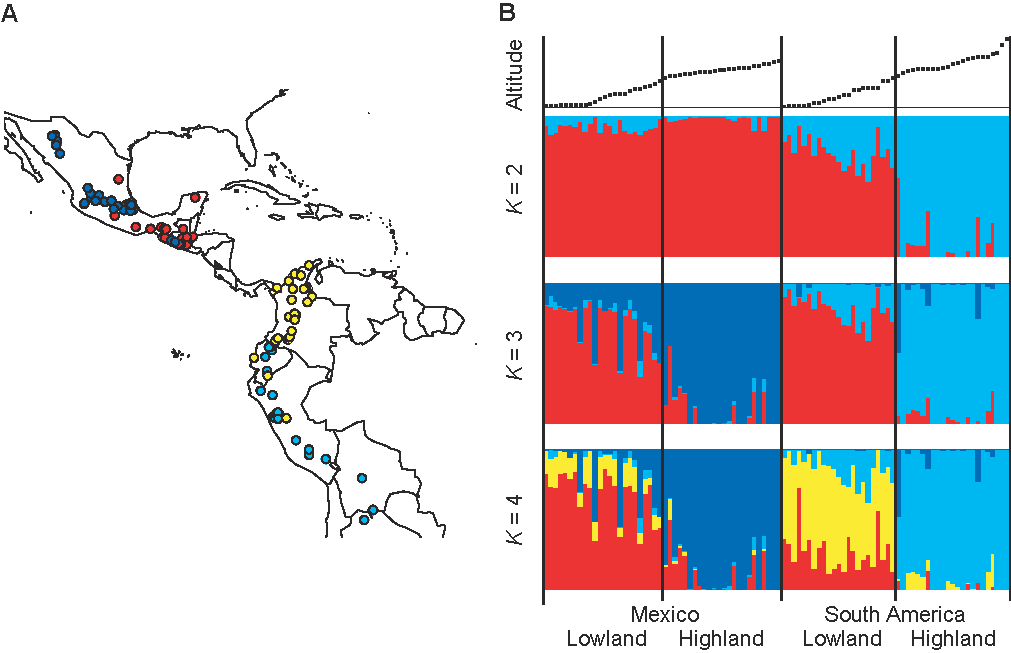
\includegraphics[width=0.8\textwidth]{fig/Fig2}
   \renewcommand{\baselinestretch}{0.9}
   \vspace{-3mm}
   \caption{(A) Sampling locations of landraces.  Red, blue, yellow and light blue dots represent Mexico lowland, Mexico highland, SA lowland and SA highland populations, respectively.  (B) Results of {\sf STRUCTURE} analysis of the maizeSNP50 SNPs with $K=2\sim4$.  The top panel shows the altitude, ranging from 0 to 4,000 m on the \emph{y}-axes.  The colors in $K=4$ correspond to those in panel (A).    }
\vspace{-6mm}
    \label{map}
  \end{center}
\end{figure*}
%%%%%%%%%%%%%%%%%%%%%%%%%%%%%%%%%%%%%%%%%% FIGURE


\section*{Materials and Methods}

\subsection*{Materials and DNA extraction}
We included one individual from each of 94 open-pollinated landrace maize accessions from high and low elevation sites in Mexico and South America (Table S1).  Accessions were provided by USDA germplasm repository or kindly donated by Major Goodman (NCState).  
Sampling locations are shown in Figure~\ref{map}A (see also supp table S1).  
%shouldn't we put table refs in case these change?
Landraces sampled from altitudes $<$1,700 m were considered lowland, while accessions from $>$1,700 m were considered highland (supp table S1).  
%Please fill in information in table S1 from Matt's excel file (dropbox).  
Seeds were germinated on filter paper following fungicide treatment and grown in standard potting mix.  Leaf tips were harvested from plants at the five leaf stage.  Following storage at $-80{}^\circ$C overnight, leaf tips were lyophilized for 48 hours.  Tissue was then homogenized with a Mini-Beadbeater-8 (BioSpec Products, Inc., Bartlesville, OK, USA).  DNA was extracted using a modified CTAB protocol \cite[]{CTAB}.  The quality of DNA was ensured using methods described in \cite{vanHeerwaarden_2011_21189301}.

\subsection*{SNP data}
We used the maize B73 genome sequence RefGen version 2 as a reference \cite[]{Schnable_2009_19965430}.  
The filtered gene set (version 5b\_FGS) was retrieved from MaizeSequence.org for SNP annotations.  
%isn't it 5b_60?
We excluded genes annotated as transposable elements (84) and pseudogenes (323) from the filtered gene set, resulting in a total of 38,842 genes.
%I think the above needs to go after the SNP50 information perhaps in separate section. we didn't use the FGS to call SNPs (Kelly may have to mention refgen2 in her section).

We generated two complementary SNP data sets for the sampled maize landraces. 
The first set was generated using the Illumina MaizeSNP50 BeadChip platform, including 56,110
SNPs \cite[]{Ganal_2011_22174790}.  SNPs were clustered with the default algorithm of the GenomeStudio Genotyping Module v1.0 (Illumina Inc., San Diego, CA, USA).   
Clustering for each SNP was then visually inspected and manually adjusted.  
These data are referred to as "MaizeSNP50" hereafter.  
MaizeSNP50 data have high reproducibility and a low proportion of missing data but are subject to ascertainment bias. 
This array contains SNPs discovered in five ascertainment schemes \cite[]{Ganal_2011_22174790}; however, the vast majority of SNPs come from two panels: the Syngenta set (14,810 SNPs), derived from polymorphisms distinguishing the parents of the IBM mapping population (the maize lines B73 and Mo17), and the Panzea set, including 40,594 SNPs identified during sequencing of the 25 parents of the NAM mapping population.  

The second data set was generated utilizing high-throughput Illumina sequencing data in a method referred to as \underline{g}enotyping-\underline{b}y-\underline{s}equencing (GBS).  \textcolor{red}{Kelly is up for details.}
Average coverage was relatively low \textcolor{red}{(XXX)}, likely resulting in heterozygotes often being miscalled as homozygotes.  However, this data set is relatively free from ascertainment bias.       
%please fill in X
GBS data were obtained for a subset of 87 of the landrace accessions (Supp. Table 1). 

To assess data quality, we compared genotypes at the 7,197 SNPs that overlap between the MaizeSNP50 and GBS data sets. 
Excluding missing data, we compared 229,937 genotypes. 
While only 0.8\% of 173,670 homozygous loci in the MaizeSNP50 data set differed from GBS genotypes, 88.6\% of 56,267 MaizeSNP50 heterozygotes had different genotypes in the GBS data, being homozygous in nearly all cases. 
Despite an extremely high heterozygote error rate, our GBS data should be informative given the high correlation in allele frequencies between data sets ($r=0.89$; Supp fig. X) and a lack of major allele or reference bias (data not shown).
%please fill in X

\subsection*{Structure analysis}
We performed {\sf STRUCTURE} analysis \cite[]{Pritchard_2000_10835412,Falush_2003_12930761} using  synonymous and noncoding SNPs from the MaizeSNP50 data. 
We assumed free recombination between SNPs without missing data and randomly pruned SNPs closer than 10 kb (alternative distances were tried with nearly identical results). 
We excluded SNPs in which the number of heterozygous individuals exceeded homozygotes and where the \emph{P}-value for departure from Hardy-Weinberg Equilibrium (HWE) based on a \emph{G}-test was smaller than 0.5\% using all individuals. 
% i removed sentence on paralogy. is "extreme heterozygosity" different from the above?
Following these data thinning measures, 17,013 biallelic SNPs remained. 
We conducted three replicate runs of {\sf STRUCTURE} using the correlated allele frequency model with admixture for \emph{K} = 2$\sim$6 populations, a burn-in length of 50,000 iterations and a run length of 100,000 iterations. 
Results across replicates were nearly identical.

\subsection*{Demographic inference}
We tested three demographic models in which maize was differentiated into high- and lowland populations subsequent to domestication (Figure~\ref{model}). 
Observed joint frequency distributions (JFDs) were calculated using the GBS data set due to its lower level of ascertainment bias. 
A subset of silent SNPs were utilized that had $\geq15$ individuals without missing data in both low- and highland populations and did not violate HWE.  
An HWE cut-off of $P<0.005$ was used for each subpopulation due to our under-calling of heterozygotes. 
In total, we included 18,745 silent SNPs for the Mexican populations in Models IA and IB, 14,508 for the South American populations in Model I and 11,305 for the Mexican lowland population and the South American populations in Model II.  
We obtained similar results under more or less stringent thresholds for significance ($P < 0.05\sim0.0005$; data not shown), though the number of SNPs was very small when $P<0.05$.  
Demographic parameters were inferred using the software {\sf dadi} \cite[]{Gutenkunst_2009_19851460}.  We calculated an expected JFD given parameters from a diffusion method and the likelihood obtained from the expected and observed JFDs in the multinomial approach of this software. \\
%any other dadi parameters etc. we need to report?

%%%%%%%%%%%%%%%%%%%%%%%%%%%%%%%%%%%%%%%%%% FIGURE
\begin{figure}[tb]   
  \begin{center}
   \vspace{-0mm}
   %\includegraphics[width=0.23\textwidth]{figs/model}
   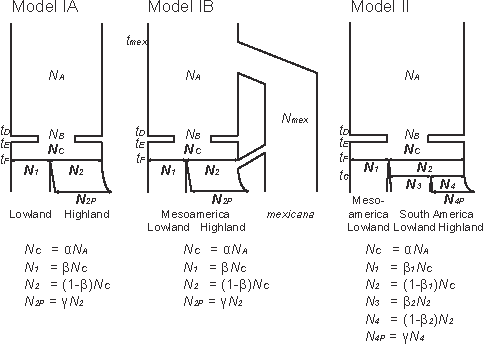
\includegraphics[width=0.5\textwidth]{fig/Fig3}
   \renewcommand{\baselinestretch}{0.9}
   \vspace{-3mm}
   \caption{ Demographic models of maize low- and highland populations.  Parameters provided in bold were estimated in this study.  See text for details.
   }
\vspace{-6mm}
    \label{model}
  \end{center}
\end{figure}
%%%%%%%%%%%%%%%%%%%%%%%%%%%%%%%%%%%%%%%%%% FIGURE

%Sho please change so it says Model 1A and 1B and II.

\subsubsection{Model IA}
This model is applied to the Mexico and SA populations.
We assume the ancestral diploid population representing \emph{parviglumis} follows a standard Wright-Fisher model with constant size.  The size of the ancestral population is denoted by $N_A$.
At $t_D$ generations ago, the bottleneck event begins at domestication, and at $t_E$ generations ago, the bottleneck ends.  The population size and duration of bottleneck are denoted by $N_B$ and $t_B=t_D-t_E$, respectively.  The population size recovers to $N_C=\alpha N_A$ in the lowlands.  
Then, the highland population is differentiated from the lowland population at $t_F$ generations ago.  The size of the low- and highland populations at time $t_F$ is determined by a parameter, $\beta$ such that the population is divided by $\beta N_C$ and $(1-\beta)N_C$.  
We assume that the population size in the lowlands is constant but that the highland population experiences exponential expansion after divergence: its current population size is $\gamma$ times larger than that at $t_F$.  \\

\subsubsection{Model IB}
We expand Model IA for the Mexico populations.  We incorporate admixture from \emph{mexicana} to the highland Mexican maize population.  The time of differentiation between \emph{parviglumis} and \emph{mexicana} occurs at $t_{mex}$ generations ago.  The size of the \emph{mexicana} population is denoted by $N_{mex}$ and this size is assumed to be constant.  At $t_F$ generations ago, the Mexico highland population is derived from the Mexico lowland population and admixture with \emph{mexicana}.  The proportion of admixture with \emph{mexicana} is denoted by $P_{mex}$.  \\

\subsubsection{Model II}
The final model is for the Mexico lowland, SA lowland and SA highland populations.  This model was used for simulating SNPs with ascertainment bias (see below).  At time $t_F$, the Mexico and SA lowland populations are differentiated, and the sizes of populations after splitting are determined by $\beta_1$.  At time $t_G$, SA lowland and highland populations are differentiated, and the sizes of populations at this time are determined by $\beta_2$.  As in Model IA, the SA highland population is assumed to experience population growth with the parameter, $\gamma$.\\


%%%%%%%%%%%%%%%%%%%%%%%%%%%%%%%%%%%%%%%%%% FIGURE
\begin{figure}[tb]   
  \begin{center}
   \vspace{-0mm}
   %\includegraphics[width=0.23\textwidth]{figs/model}
   \includegraphics[width=0.5\textwidth]{fig/Fig4}
   \renewcommand{\baselinestretch}{0.9}
   \vspace{-3mm}
   \caption{Observed and expected joint distributions of minor allele frequencies in low- and highland populations in (A) Mexico and (B) South America. }
\vspace{-6mm}
    \label{JFD}
  \end{center}
\end{figure}
%%%%%%%%%%%%%%%%%%%%%%%%%%%%%%%%%%%%%%%%%% FIGURE

Estimates of a number of our model parameters were available from previous work.    
$N_A$ was determined using estimates of the composite parameter $4N_A\mu$ and a separate estimate of mutation rate, $\mu$, per site per generation.  $4N_A\mu$ was estimated in \emph{parviglumis} to be $\sim$0.018  \cite[]{Eyre-Walker_1998_9539756,Tenaillon_2001_11470895,Tenaillon_2004_15014173,Wright_2005_15919994,Ross-Ibarra_2009_19153259}.  
The mutation rate in maize has been estimated to be $2.9\sim 3.3\times 10^{-8}$, so we assume $\mu=3\times 10^{-8}$ \cite[]{Clark_2005_16079248}.  
Thus, $N_A$ was set to $0.018/4/(3\times 10^{-8}) = 150,000$.
The severity of the domestication bottleneck is represented by $k=N_B/t_B$ \cite[]{Eyre-Walker_1998_9539756,Wright_2005_15919994}, and following \cite{Wright_2005_15919994} we assumed $k=2.45$ and $t_B=1,000$ generations.  
Taking into account archaeological evidence \cite[]{Piperno_2009_19307570}, we assume $t_D=9,000$ and $t_E=8,000$.  
We further assumed $t_F=6,000$ for Mexican populations in Models IA and II \cite[]{Piperno_2006_69}, $t_F=4,000$ for South American populations in Mode lI \cite[]{Perry_2006_16511492}, and $t_{mex}=60,000$, $N_{mex}=160,000$ \cite[]{Ross-Ibarra_2009_19153259}, and $P_{mex}=0.2$ \cite[]{vanHeerwaarden_2011_21189301} for Model IB. 
For both Models IA and IB, we inferred three parameters ($\alpha$, $\beta$ and $\gamma$), and, for Model II, we fixed $t_F=6,000$ and $t_G=4,000$ \cite[]{Piperno_2006_69,Perry_2006_16511492} and estimated the remaining four parameters ($\alpha$, $\beta_1$, $\beta_2$ and $\gamma$).

\subsection*{Differentiation between low- and highland populations}
We used our inferred demographic model to generate a null distribution of $F_{ST}$ via simulation using the software {\sf ms} \cite[]{Hudson_2002_11847089}.   
The command line options for {\sf ms} are provided in supp Table 2.  Generating the null distribution of differentiation for the MaizeSNP50 data requires accounting for ascertainment bias. Evaluation of genetic clustering in our data (not shown) coincides with previous work \cite[]{Hufford_2012_22660546} in suggesting that the two lines most important in the ascertainment panel are most closely related to Mexican lowland maize.  
We thus added two additional individuals to the Mexican lowland population and generated our null distribution using only SNPs for which the two individuals had different alleles. For model IA in South America we added two individuals at time $t_F$ to the ancestral population of the South American low- and highland populations because the Mexican lowland population was not incorporated into this model. For each combination of sample sizes in low- and highland populations, we generated $10^7$ $F_{ST}$ values and used these as a null distribution in order to evaluate our data.   We calculated $F_{ST}$ values for all SNPs that had $\geq10$ individuals with no missing data in all four populations and showed no departure from HWE at the 0.5\% (GBS) or 5\% (MaizeSNP50) level. 

\subsection*{Haplotype scoring test}
We performed a \underline{p}airwise \underline{h}aplotype \underline{s}coring (PHS) test to detect further evidence of selection, following \cite{Toomajian_2006_16623598}.  
To conduct this test, we first imputed and phased the combined SNP data (both GBS and MaizeSNP50) using the {\sf fastphase} software ver. 1.4.0 \cite[]{Scheet_2006_16532393}.  
As a reference for phasing, we used data (excluding heterozygous SNPs) from an Americas-wide sample of 23 partially inbred landraces that were included in the Hapmap v2 data set  \cite[]{Hufford_2012_22660546}.  
%should really cite Chia here instead of Hufford. 
{\sf fastphase} was run with default parameter settings.  PHS was calculated for an allele \emph{A} at position $x$ by

\begin{equation}
  \label{phs-1}
  \begin{array}{l}
  \displaystyle{
PHS_{x_A} = \sum^{p-1}_{i=1}\sum^{p}_{j=i+1}Z_{ijx}  / \Bigl( \begin{array}{c} p \\ 2 \\ \end{array} \Bigr) 
- \sum^{n-1}_{i=1}\sum^{n}_{j=i+1}Z_{ijx}  / \Bigl( \begin{array}{c} n \\ 2 \\ \end{array} \Bigr) 
  }
  \end {array} 
  \textrm{,}
\end{equation}

\noindent where $n$ is sample size of haploids, $p$  is the number of haploids carrying the allele $A$ at position $x$, and

\begin{equation}
  \label{phs-2}
  \begin{array}{l}
  \displaystyle{
Z_{ijx} = \frac{ d_{ijx} - \bar{d_{ij}} }{ \sigma_{ij} }
  }
  \end {array} 
  \textrm{,}
\end{equation}

\noindent where $d_{ijx}$ is the genetic distance over which individuals $i$ and $j$ are identical surrounding position $x$, $\bar{d_{ij}}$ is the genome-wide mean of distances over which individuals are identical, and $\sigma_{ij}$ is the standard deviation of the distribution of distances.  
The \emph{P}-value for an allele $A$ with frequency $p$ at position $x$ was calculated such that Pr($PHA_{xA}\leq PHA_{null|p}$), where $PHA_{null|p}$ are the PHS values for all alleles with frequency $p$ across the genome. 
%is $PHA_{p}$ a mean? The previous sentence needs to be clarified.

Genetic distances were obtained from the IBM mapping population \cite[]{Ganal_2011_22174790}.  
While genetic positions were initially only available for the MaizeSNP50 data set, we fit genetic (cM) and physical (bp) distances to a tenth degree polynomial curve, and calculated cM for all SNPs. 
%please provide the genetic map positions for all SNPs. probably not needed in the paper, but I would like this data.
 
%%%%%%%%%%%%%%%%%%%%%%%%%%%%%%%%%%%%%%%%%% FIGURE
\begin{figure}[tb]   
  \begin{center}
   \vspace{-0mm}
   %\includegraphics[width=0.23\textwidth]{figs/model}
   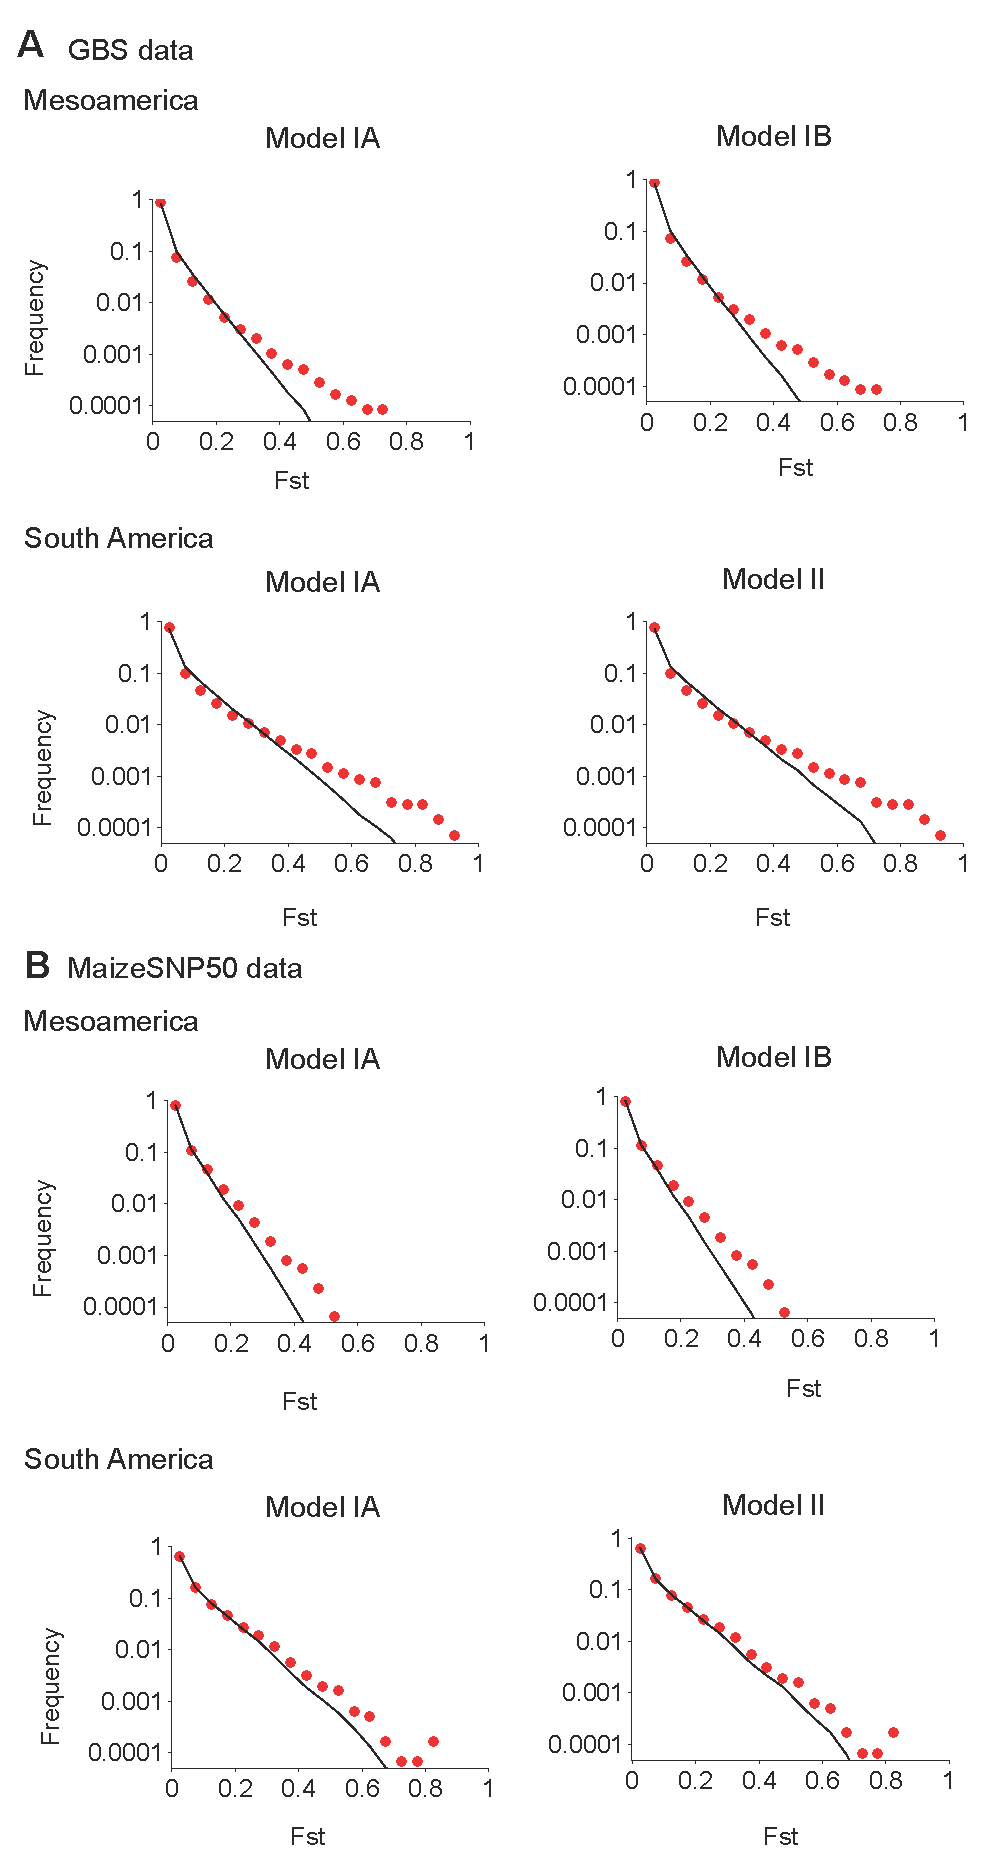
\includegraphics[width=0.45\textwidth]{fig/Fig5}
   \renewcommand{\baselinestretch}{0.9}
   \vspace{-3mm}
   \caption{Observed and expected distributions of $F_{ST}$ values in GBS (A) and MaizeSNP50 data (B).  The \emph{x}-axes represent $F_{ST}$ values.  The \emph{y}-axes represent the frequency of SNPs with $F_{ST}$ values within a bin of 0.05 size.  Red dots and solid lines indicate observed and expected distributions. 
   }
\vspace{-6mm}
    \label{FstDist}
  \end{center}
\end{figure}
%%%%%%%%%%%%%%%%%%%%%%%%%%%%%%%%%%%%%%%%%% FIGURE


%%%% PLR:
\subsection*{Theoretical valuation of parallel adaptation }

We suggest below that many of these high-$F_{ST}$ alleles are locally adaptive,
and the degree of coincidence between highland regions informs us about 
whether these adaptations occurred indpendently (in parallel), or if alleles transited between the two.
To see if the abundance and degree of coincidence is consistent with what is known about the population history of maize,
we evaluated the rate at which we expect an allele that provides a selective advantage at higher altitude
to arise by new mutation in a highland region ($\mutrate$),
and the rate at which such an allele already present in the Mexican highlands
would transit the intervening lowlands and fix in the Andean highlands ($\migrate$). 
In each case we assume alleles adaptie in the highland are slightly deleterious at lower altitude.
These numbers depend most strongly on the population density, 
the selection coefficient,
and the rate at which seed is transported long distances and replanted.
We evaluated these rates using new and existing theory, and validated by simulation.

%Matt please add a few lines (cite Mercer?) about why we assume deleterious

To calculate the rate at which new mutations appear and fix in the highland population, $\mutrate$,
we multiplied the total population size of the highlands by the mutation rate per generation
and by the chance that a single such mutation successfully fixes
(i.e.\ is not lost to drift).
The latter probability, that a single new mutant allele providing benefit $s_b$ to heterozygotes at high elevation
will increase in frequency and fix in the high elevation patch,
is approximately $2s_b$ divided by the variance in offspring number \citep{jagers1975branching}.
This is not quite right, since such a mutation could occur at low elevation,
where it is deleterious,
and its offspring could then migrate to high elevation and fix there.
%but we use this assumption anyway?
Similarly, if we use the selection coefficient for high elevation,
this ignores the fact that some of the seeds from the high-elevation plants may be grown at low elevation,
reducing the chance of fixation of an allele that appears at high elevation.
This scenario has been well-studied in theoretical models by \citet{polk} and \citet{barton1987establishment},
% missing reference for Polk.
but it is not immediately obvious how well their approximations apply to maize 
as it grows across an altitudinal gradient (rather than an abrupt transition) and has high variance in number of offspring.
Therefore, we used the following more detailed demographic model (following \citet{vanHeerwaarden2010}) 
%cite van Heerwaarden  2010 Heredity
to numerically calculate the chance of fixation of a beneficial allele
as a function of the location it first appears.
We found that the simple approximation is quite good,
although the demographic model was necessary to find the variance in offspring number,
as well as the migration rate, which we will need later.

%TODO: describe demographic model in words.  (including migration which we need later.)
%Reference math and more detail in appendix.

\plr{could alternatively: (a) describe the math; or (b) cut this down further.}
%I actually like this as is, but think we should expand math as separate appendix. my thinking is math will be of interest to a subset of audience, so perhaps best presented fully but at end. thoughts?

Concretely, the probability that a new mutation destined for fixation
will arise in a patch of high-elevation habitat of area $A$ in a given generation
is a function of the density of maize per unit area $\rho$,
the selective benefit $s_b$ it provides,
the mutation rate $\mu$,
and the variance in offspring number $\xi^2$.
In terms of these parameters, the rate of appearance is
\begin{align} \label{eqn:mutrate}
  \mutrate = \frac{2 \mu \rho A s_b}{\xi^2} .
\end{align}

A corresponding expression for the chance that an allele moves from one highland population to another is harder to intuit,
and is addressed in more depth in \citep{ralphcoop2013patches}.
If an allele is beneficial at high elevation, and fixed in the Mexican highlands,
but deleterious at low elevations,
then it will be present at low frequency in nearby lowland populations,
maintained at migration-selection balance \citep{slatkin1973geneflow}.
This equilibrium frequency decays exponentially with distance,
so that the highland allele is present at distance $R$ from the highlands at frequency $C \exp(- R \sqrt{2s_m} / \sigma)$,
where $s_m$ is the deleterious selection coefficient for the allele in low elevation,
$\sigma$ is the mean dispersal distance (mean distance between parent and offspring),
and $C$ is a constant depending on geography ($C\approx 1/2$ is close).
Multiplying this frequency by a population size gets the predicted number (average density across a large number of generations) of individuals carrying the allele in that population.
Therefore, in a lowland population of size $N$ at distance $R$ from the highlands,
$(N/2)  \exp(- R \sqrt{2s_m} / \sigma)$ is equal to the probability that there are any highland alleles present,
multiplied by the expected number of these, given that there are some present.
Since the latter is at least 1,
%don't follow. "latter" is expected number? why is that at least one? didn't you say above it could be 0<x<1 because it's an average density?
the chance there are any present in a given generation is no more than $(N/2) \exp(- R \sqrt{2s_m} / \sigma)$,
and so this puts an upper bound on $\migrate$.
Therefore, we would need to wait around $\Tmig = (2/N)\exp(R \sqrt{2s_m} / \sigma)$ generations 
for a rare such excursion to occur.
Concretely, we can use that
\begin{align}
  \migrate \le (N/2)  \exp(- R \sqrt{2s_m} / \sigma) ,
\end{align}
with $N$ the total size of the unadapted highland population,
and $R$ the distance from the adapted to the yet-undapted highland populations.
Another factor this omits is the probability that such an allele fixes ($\approx 2s_b/\xi^2$), but since such alleles arrive by migration this omission is unlikely a large effect and is conservative.
%Peter please check if simplification to sentence above OK. OK to include \approx?

To obtain specific predictions,
we then computed $\mutrate$ and $\migrate$ at various parameter values.
We also checked these with simulations and more detailed computations,
described in the Appendix.


\section*{Results and Discussion}

%%%%%%%%%%%%%%%%%%%%%%%%%%%%%%%%%%%%%%%%%%%%%%%%%%%%%%%%%%%%
\renewcommand{\arraystretch}{1.1}
\begin{table}[tb]

\begin{center}
 \caption[]{Silent site $F_{ST}$ from GBS SNPs \hspace*{2.3cm}}
  \textbf{}\\[-2mm]
{\fontsize{7}{9}\sf
    \begin{tabular}{llccccccl}
    \hline
    & & \\[-3mm]
	&		&	\multicolumn{2}{c}{Mexico}		&	\multicolumn{2}{c}{South America}		\\
	&		&	Lowlands	&	Highlands	&	Lowlands	&	Highlands	\\
      \hline
    & & \\[-3mm]
Mexico	&	Lowlands	&	--	&		&		&		\\
	&	Highlands	&	0.0244	&	--	&		&		\\
SA	&	Lowlands	&	0.0227	&	0.0343	&	--	&		\\
	&	Highlands	&	0.0466	&	0.0534	&	0.0442	&	--	\\ [1mm]
    \hline
    \end{tabular}
    \label{FstP}  % caption is needed to make this work
}
\end{center}
\end{table}
\renewcommand{\arraystretch}{1}
%%%%%%%%%%%%%%%%%%%%%%%%%%%%%%%%%%%%%%%%%%%%%%%%%%%%%%%%%%%%

%Matt, please add a sentence or two at the start say "we sampled X, genotyped using Y etc.?? You can use stats from the paragraph below on total number of SNPs
%MBH: So this is already in the Methods.  Do we need to recapitulate here?
%Sho, please move some of the other numbers below (SNPs tested etc.) to methods.
%
%\subsubsection{Joint data set}In total, 91,779 SNPs remained in our joint, filtered GBS and MaizeSNP50 data set ($2n\geq20$ and HWE $P\geq0.005$ \mbh{need to keep track of how this is reported: sometimes 0.005, sometimes 0.5\%} for GBS or $P\geq0.05$ for MaizeSNP50 for all four populations).  For the Mexican and South American populations, we calculated \emph{P}-values for 76,989 and 63,160 SNPs respectively with the remaining SNPs being monomorphic. The reduced number of polymorphic SNPs in South America relative to Mexico is likely due to a lower effective population size in the South American populations.  48,370 SNPs were polymorphic in both Mexico and South America. 

\subsection*{Population structure}

We performed a {\sf STRUCTURE} analysis \cite[]{Pritchard_2000_10835412,Falush_2003_12930761} of our landrace sample, varying the number of groups from $K=2\sim 6$ (Figure \ref{map}, Supp FigX). 
%cite supp. figure with likelihood plot from STRUCTURE
Most landraces were assigned to groups consistent with \emph{a priori} population definitions, but admixture between highland and lowland populations was evident at intermediate elevations ($\sim1700$m).  Consistent with previously described scenarios for maize diffusion \cite[]{Piperno_2006_69}, we find evidence of shared ancestry between lowland Mexican maize and both Mexican highland and South American lowland populations.  Pairwise $F_{ST}$ among populations reveals low overall differentiation (Table \label{FstP}), and the higher $F_{ST}$ values observed in S. America are consistent with decreased admixture seen in STRUCTURE.  Archaeological evidence supports a more recent colonization of the highlands in S. America  \cite[]{Piperno_2006_69,Perry_2006_16511492,Grobman_2012_22307642}, suggesting that the observed differentiation may be the result of a stronger  bottleneck during colonization of the S. American highlands. 

\subsection*{Population differentiation under inferred demography}

To provide a null expectation for allele frequency differentiation, we used the joint site frequency distribution (JFD) of lowland and highland populations to estimate parameters of two demographic models (Fig.~\ref{model}) using the maximum likelihood method implemented in {\sf dadi} \cite[]{Gutenkunst_2009_19851460}.  
Estimated parameter values are listed in Table~\ref{param}; while the observed and expected JFDs were quite similar for both models,  residuals indicated an excess of rare variants in the observed JFDs in all cases (Fig.~\ref{JFD}). 
%parameter table now in supplement.
Under both models IA and IB,  we found expansion in the highland population in Mexico to be unlikely, but a strong bottleneck followed by population expansion is supported in S. American maize in both models IA and II.  
The likelihood value of model lB ($-$4641.28) was much higher than the likelihood of model IA ($-$5590.33) (Table~\ref{param}), consistent with analyses suggesting that introgression from \emph{mexicana} played a significant role during the spread of maize into the Mexican highlands \cite{Profford_2013}. 

In addition to the parameters listed in Fig.~\ref{model}, we investigated the impact of varying the domestication bottleneck size ($N_B$).  
Surprisingly, $N_B$ was estimated to be equal to $N_C$, the population size at the end of the bottleneck, and the likelihood of $N_B<N_C$ was much smaller than for alternative parameterizations (Table~\ref{param}, supp table~3) 
%please go through and check we have these supp. tables and they are cited in the correct order.
This result appears to contradict earlier work using sequences from coding regions to infer a maize domestication bottleneck \cite{Wright_2005_15919994, Tenaillon2004}.  One explanation for this discrepancy may be the action of purifying selection in coding regions, which could act to retard the recovery of diversity and lead to estimates of a stronger bottleneck \cite{Hufford_2012_22660546}.  Consistent with \citet{Hufford_2012_22660546}, our genome-wide SNP data show an excess of rare variants relative to expectations under \cite{Wright_2005_15919994}'s bottleneck model (Fig.~\ref{JFD}), suggesting a domestication model involving a weaker bottleneck or more rapid population growth.
% Peter does more rapid pop growth make sense? I don't think it's really more rapid, I think it's just that the lack of rare variants in coding regions leads to over-estimation of bneck strength. Is that plausible (graham seemed skeptical when I mentioned this).

Comparing our empirical $F_{ST}$ values to the null expectation simulated under our demographic models allowed us to identify significantly differentiated SNPs between low- and highland populations. In all cases, observed $F_{ST}$ values were quite similar to those generated under our null models  (Figure~\ref{FstDist}A)), and model choice -- including the parameterization of the domestication bottleneck -- had little impact on the distribution of estimated of p-values (Supp Figure~4). We chose $P<0.01$ as an arbitrary cut-off for significant differentiation between low- and highland populations, and identified 1,040 SNPs in Mexico (1,040/76,989=0.0135) and 756 SNPs in South America (756/63,160=0.0120) as outliers.  

%\subsubsection{MaizeSNP50 data} Without this modification of our demographic model, we underestimated \emph{P}-values, but the effect was very small (Supp Figure~6).   Furthermore, the empirical and null distributions of $F_{ST}$ values were very similar in the MaizeSNP50 data set despite the fact that multiple ascertainment schemes were used (Figure~\ref{FstDist}B; Supp Figure~6). 
%
%I vote to delete the above commented out section. we do the correction, so no need to say it's a small effect if we don't do it right?

%%%%%%%%%%%%%%%%%%%%%%%%%%%%%%%%%%%%%%%%%% FIGURE
\begin{figure}[tb]   
  \begin{center}
   \vspace{-0mm}
   %\includegraphics[width=0.23\textwidth]{figs/model}
   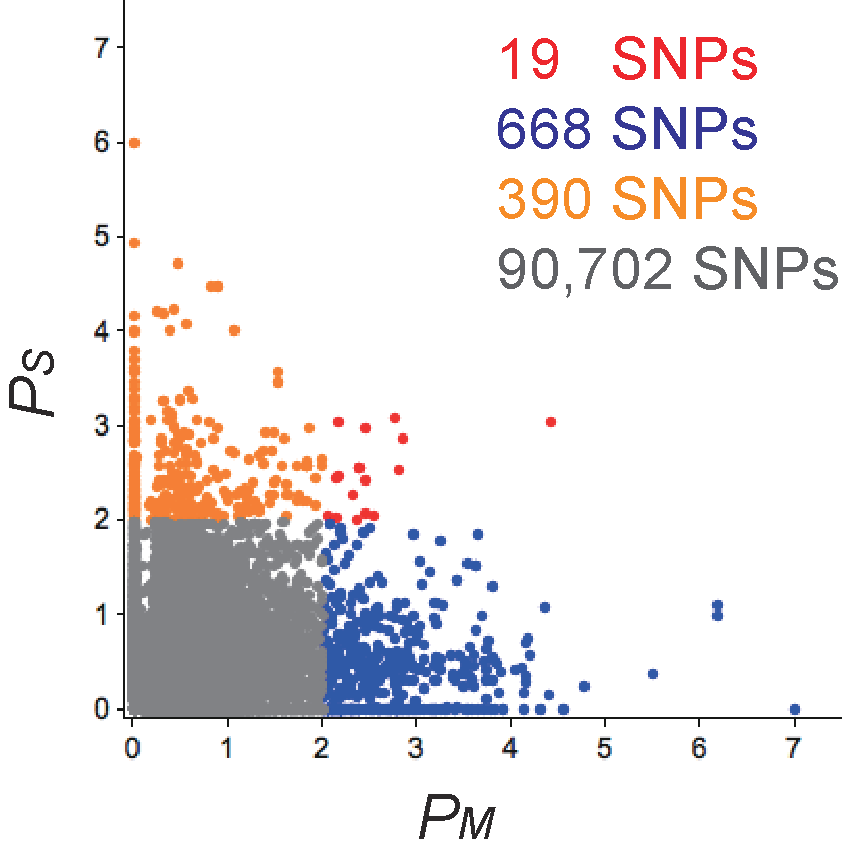
\includegraphics[width=0.4\textwidth]{fig/Fig6}
   \renewcommand{\baselinestretch}{0.9}
   \vspace{-3mm}
   \caption{Scatter plot of $F_{ST}$ \emph{P}-values in Mexico ($P_M$ on \emph{x}-axes) and South America ($P_S$ on \emph{y}-axes).  $P_M$ and $P_S$ are scaled by --log$_{10}$.  Red, blue, orange and gray dots represents SNPs showing significance in both Mexico and South America, only in Mexico, only in South America, respectively (see text for details).} 
\vspace{-6mm}
    \label{PvDist}
  \end{center}
\end{figure}
%%%%%%%%%%%%%%%%%%%%%%%%%%%%%%%%%%%%%%%%%% FIGURE
%
%do we know what that clear outlier red SNP is? anything interesting?

\subsection*{Patterns of adaptation}

\subsubsection{Adaptation via mutation versus standing variation}

In order to characterize patterns of adaptation, we first determined whether  SNPs showing high differentiation between the lowlands and the highlands arose primarily through new mutations or standing genetic variation.  
We found that these putatively adaptive variants in both Mexico and South America tended to segregate in lowland populations more often than other SNPs (84.6\% vs. 74.8\% in Mexico, FET {$P < 10^{-11}$ and 87.3\% vs 81.8\% in South America,  $P< 10^{-3}$).  We extended this analysis to standing variation in \emph{parviglumis} by retrieving SNP data from 14 \emph{parviglumis} inbred lines included in the Hapmap v2 data set, using only SNPs with $n\geq10$ \cite[]{Hufford_2012_22660546}.  Again we found that putatively adaptive variants were more likely to be polymorphic in \emph{parviglumis} (81.1\% vs. 72.1\% in Mexico, FET {$P < 10^{-6}$ and 81.2\% vs 72.7\% in South America,  $P< 10^{-4}$).  
%MBH: Sho, I extensively edited the previous sentences of this paragraph.  I was careful to keep all \%'s and $P$-values straight, but might be a good idea to double check

These results suggest that maize adaptation to high altitudes has largely made use of standing genetic variation. 
%etc.evidence for selection from standing variation is increased in model organisms such as Drosophila (Petrov arXiv) and human \cite[]{Turchin_2012_22902787,Peter_2012_23071458}.}
%Sho: please add a sentence or two here on other empirical results on standing var (including the above). We also need a sentence or two here on why we expect this based on theory. I think we drop the domestication comparison
Because linkage disequilibrium in maize decays rapidly (CITE), it is plausible that a number of hard sweeps -- strong selection on new mutations -- would be missed by our data, but several lines of evidence suggest to us that this is unlikely.  
%Guys, help here.  My thinking is:
% 1) we see few private SNPs (true? I didn't quite understand your email Sho. what % of SNPs are unique to a population when we include teosinte?
% 2) We do see evidence of selection on other SNPs (at least high Fst), suggesting that even if there are hard sweeps we missed, a substantial amount of selection on standing var appears to have occurred.
% 3) The number of hard sweeps couldn't have been huge or we would see some.
% We need to summarize whether we believe the missed hard sweeps idea is likely or not in a few sentences. Sho, what do you think? Take a stab at it?

\subsubsection{Highland versus lowland adaptation}  

Given the historical spread of maize from an origin in the lowlands, it is tempting to assume that significant population differentiation should be primarily due to an increase in frequency of adaptive alleles in the highlands.
To test this hypothesis, we sought to identify the adaptive allele at each locus using comparisons between Mexico and South America as well as to \emph{parviglumis} (Supplemental methods).
%
%I think these bar graphs and explanation should go in the supplement. Opinions?
%MBH:I think the edits below improve the narrative, but they gut the results; it makes it easy on the reader that just wants to trust us on the details, but personally I would want more details before I'd buy these results and then I'd be annoyed that I had to dig through the supplement in order to get them.
%
%However, we cannot rule out the possibility of adaptation in the lowlands.
%Therefore we further investigated patterns of allele frequency change across populations.
%When data were available for \emph{parviglumis} from Hapmap v2 \cite[]{Chia_2012_22660545,Hufford_2012_22660546}, we included these in our analysis.
%
%First, we assessed patterns of allele frequencies in SNPs that were significantly differentiated between highland and lowland maize.
%We focused on SNPs segregating as shown in Fig.~\ref{tes2}A, although some SNPs showed more complex patterns.
%The first and second rows show hypothesized patterns of segregation under highland adaptation; here, allele frequencies in maize from a highland region are highly differentiated from those of \emph{parviglumis} and maize from the corresponding lowland region. %and no difference is observed between South America populations.
%When \emph{parviglumis} data are lacking, SNPs showing the pattern of segregation in the third row likely underly highland adaptation.
%\mbh{don't think this row in the figure is necessary}
%Similarly, patterns of SNP segregation depicted in the fourth to sixth rows are consistent with lowland adaptation.
%The patterns expected for highland and lowland adaptation in South America are qualitatively the same as those shown for Mexico in Fig.~\ref{tes2}A.
%
Consistent with predictions, we infer that differentiation at X\% (537) and Y\% (530) of SNPs in Mexico and South America is due to adaptation in the highlands, with only A\% and B\% of SNPs inferred to be due to lowland adaptation. The majority of these SNPs show patterns of haplotype variation consistent with our inference (Supp. Table X).
%This supp. table should show numbers and % of PHS stats and allele segregation patterns. Easier to parse in a table.
%
%inferred to be adapted in highland or lowland environments showe(74.5\% in Mexico and 84.5\% in South America) of putatively highland-adaptive SNPs also had lower P-values for the PHS test in highland maize. 
%Likewise, 63.5\% and 67.1\% of the putatively adaptive SNPs in Mexico and South America that showed segregation patterns consistent with lowland adaptation also showed lower P-values for the PHS test in lowland maize.
%Additionally, when a putatively derived allele segregated in both the lowlands and highlands but was more prevalent in the highlands, 67.5\% and 67.6\% of such SNPs showed lower PHS \emph{P}-values in the highlands in Mexico and South America. 
%\comst{I tested: $P<10^{-11}, < 0.01$, $\approx 0$, $<10^{-9}$ for Mex high, Mex low, SA high and SA low, respectively}

\subsubsection{Adaptation through introgression}

A marked difference between highland adaptation of maize in Mexico and South America is the potential for adaptation through introgression from wild relatives.  While maize in Mexico grows in sympatry with both the lowland taxon \emph{parviglumis} and the highland taxon \emph{mexicana}, maize in South America is outside the range of wild \emph{Zea} species.
 \cite{Pyhajarvi2013} recently assessed the potential for local adaptation in \emph{parviglumis} and \emph{mexicana} populations, characterizing differentiation between these subspecies using an Fst-outlier approach.
We observed a significant excess of overlap between our putatively adaptive SNPs in Mexican maize and those identified in the \cite{Pyhajarvi2013} analysis (Table~\ref{tanja}; $P<0.01$ by FET). Similar to that paper, we also find that SNPs with significant $F_{ST}$ $P$-values are enriched in intergenic regions compare to non-sigificiant SNPs (51.3\% vs. 44.2\%; FET $P < 10^{-8}$). Significant overlap was also observed between signficant SNPs in South American and teosinte ($P<0.01$), but the proportion of SNPs was lower than observed in Mexico.  These data suggest that adaptations in Mexican maize may have been obtained through gene flow with wild relatives.  To more fully explore this hypothesis we evaluated our data in light of introgression identified by \cite{Profford_2013} from \emph{mexicana} into maize in the Mexico highlands.  
The proportion of significant SNPs in introgressed regions in Mexico is significantly higher than found in South America (Fisher's exact test, $P\ll0.001$).
%When focusing on GUs, we identified 99/586 (14.5\%) and 22/466 (4.7\%) GUs of Mexico- and SA-specific significance in introgressed regions (Fisher's exact test, $P<10^{-6}$). 
%Would the genetic unit numbers work in the tanja table? i liek those numbers and think we should keep if possible.
Outside introgressed regions, the Mexican and South American populations did not show marked differences in the proportion of significant SNPs (Fisher's exact test, $P>0.7$). These results add to those of \cite{Profford_2013}, suggesting that SNPs in the introgressed regions identified have indeed been under selection.  

\subsubsection{Evidence for parallel adaptation}

While maize adaptation in Mexico and South America are likely distinguished by unique histories of gene flow with wild relatives, the potential remains for parallel adaptation in these two regions.  
SNPs showing significant differentiation between low- and highland populations in both Mexico and South America are likely candidates for parallel adaptation. 
We identify 56 SNPs with $F_{ST}$ p-values in Mexico ($P_M$) and South America ($P_S$) both $<0.01$.   
This number  was significantly larger than the random expectation ($48,370\times 0.01 \times 0.01 \approx 4.8$; $\chi^2$-test, $P\ll0.001$).  Furthermore, the distribution of $P_M$ in the 712 SNPs with $P_S<0.01$ was highly skewed toward zero (supp fig~7A), and a similar tendency was observed in $P_S$ given $P_M<0.01$ (935 SNPs; supp fig~7B).  Thus, we converted the \emph{P}-values in one population given $P<0.01$ in the other population into \emph{q}-values.  
At a false discovery rate of 0.2 we found 117 SNPs with $P_M<0.01 \cap P_S < 0.0169$ or $P_M<0.0247 \cap P_S < 0.01$, and these SNPs were considered our candidates for parallel adaptation.
We found 959 SNPs showing significant population differentiation only in Mexico ($P_M<0.01 \cap P_S > 0.0169$) and 664 SNPs only in South America  ($P_M>0.0247 \cap P_S < 0.01$).  The scatter plot of $P_M$ and $P_S$ is shown in Fig.~\ref{PvDist}.  
For a subset of 67 of the SNPs showing putative evidence of parallel adaptation candidates we also had data from \emph{parviglumis} and were able to infer based on patterns of segregation whether these SNPs were potentially adaptive under lowland or highland conditions.  Surprisingly, SNPs identified as targets of parallel adaptation in Mexico and South America more frequently show segregation patterns consistent with lowland adaptation (62 SNPs) than highland adaptation (5 SNPs). %add p-value for this comparison?
%70\% and 39.5\% of SNPs showed consistent patterns in the PHS tests in high- and lowland populations, respectively.
%Not sure what these PHS values are referring to? Do we need to keep them?
%
%Without data from \emph{parviglumis}, it is very difficult to decipher whether a segregation pattern is consistent with high- or lowland parallel adaptation.  
%\st{In total, 1,740 SNPs showed the signature of selection both or either in Mexico and South America} \
%
%Can we just skip the above commented-out text?
%
In addition to evaluating parallel adaptation at the SNP level, we investigated how often different SNPs in the same gene may have been targeted by selection. To search for this pattern, we asked whefor the target of adaptation. 
%MBH: Not sure what happened to the previous sentence.
We define a "genetic unit" or GU as all SNPs within 10kb of a transcript.  SNPs in an miRNA or second transcript within 10kb of the transcript of interest were excluded.  
We classified SNPs showing significance in Mexico, South America or in both regions into 1,277 GUs. 
Of these, 95 GUs contained at least one SNP with a pattern of differentiation suggesting parallel adaptation, whereas only 12 GUs contained both Mexico-specific and SA-specific significant SNPs. 
%I don't understand what these 95 show. 1 significant and one nonsignficiant SNP? whereas the 12 are significant in both?
Overall, fewer GUs showed evidence of parallel adaptation than expected by chance ($P<10^{-5}$), with more than 700 and 470 GUs showing Mexico-specific and SA-specific significant SNPs, respectively.  
Despite similar phenotypes and environments, we thus see little evidence for parallel adaptation at either the SNP or the gene (GU) level.  
This contrasts with data from humans \cite{Tennessen_2011_21698142} showing frequent evidence of selection on the same genes in multiple pairs of tropical and temperate human populations.  
%Points for discussion (add/delete etc.)
%genomic architecture differences? local adaptation uses regulary in teo (cite Tanja)? But what about Fraser (finds same in humans)
% More likely: taget siez



%perhaps below should be moved to methods or supp? seems out of place here.
%First, we randomly picked 959 and 664 SNPs that represent Mexico- and SA-specific differentiation (see above) from 91,779 positions and counted the number of GUs under Pattern C.

%this needs to ve moved
%CUTME
%While some have hypothesized that pre-adapted highland maize was transported through Central America to the Andes based on analysis of the \emph{Adh2} locus \cite[]{Freitas_2003_68}, analysis of larger sets of molecular markers suggests \emph{de novo} highland adaptation in South America \cite[]{Vigouroux_2008_21632329,vanHeerwaarden_2011_21189301}.  Our result of rare parallel adaptation may be consistent with independent origins of highland populations, not gene flow between the two highland populations.

%JRI stops

%Fig.~\ref{tes2}B shows the segregation patterns expected under parallel adaptation in the highlands and the lowlands.
%If there is not teosinte data, we cannot distinguish between high- and lowland adaptation.
%Surprisingly, SNPs identified as targets of parallel adaptation in Mexico and South America more frequently show segregation patterns consistent with lowland adaptation (62 SNPs) than highland adaptation (5 SNPs).
%70\% and 39.5\% of SNPs showed consistent patterns in the PHS tests in high- and lowland populations, respectively.

%Without data from \emph{parviglumis}, it is very difficult to decipher whether a segregation pattern is consistent with high- or lowland parallel adaptation.  

\subsection*{Comparison to theory}
%\plr{need discussion of choices of selection coefficients?}

% # \mutrate computation:
% A <- 500; rho <- 5000; sb <- 10^(-(1:4)); xisq <- 50
% sapply( 10^c(-5,-8), function (mu) mu * (2 * rho * A * sb)/xisq )

As a final analysis, we sought to assess whether  SNP data reveal little evidence for parallel adaptation between Mexico and S. America. Computing the rate $\mutrate$ at which newly adapted alleles arise in the population,
with a total population of $A \rho = 2.5 \times 10^6$ and an offspring variance of $\xi^2 = 50$,
we get that even if there is strong selection for the allele at high elevation ($s_b=0.1$),
then a single-base mutation with mutation rate $\mu=10^{-8}$ would still take at least 10,000 generations to appear and fix.
On the other hand, a kilobase-sized target with mutation rate $\mu=10^{-5}$
with this selection coefficient would fix in only 10 generations,
while more weakly selected alleles with $s_b$ of $10^{-2}$ or $10^{-3}$ would take hundreds or thousands of generations, respectively.
(note: at these values $\Tmut = 1/\mutrate = \mu s_b \times 10^5$.)

% # Tmig computation:
% A <- 500; rho <- 5000; sm <- 10^(-(1:4)); xisq <- 50; sigma <- 2
% 1/(sqrt(2*sm)/sigma)
% sapply( 1000*(1:4), function (R) 1 / ( A * rho * ( sqrt(2*sm) / xisq ) * exp(- sqrt(2*sm)*R/sigma ) ) )
% Ne <- (561/10^5)*A*rho 
% Ne  # = 14025
% sapply( 1000*(1:4), function (R) 1 / ( Ne * exp(- sqrt(2*sm)*R/sigma ) ) )

From the demographic model above
we have estimated that $\sigma \approx 2$ kilometers per generation,
so with $10^{-1} \ge s_m \ge 10^{-4}$ the distance $\sigma/\sqrt{2s_m}$ over which \eqref{eqn:migrate} decays 
is still short: between 4 and 150 kilometers.
\plr{put bounds on $\sigma$}
The area of the Andean highlands is about 500 km$^2$ \plr{is this right???}
which we estimate would be planted from around $N=14,000$ plants each year \plr{add more details here or above}.
Since the Mexican and Andean highlands are around 4,000 km apart,
at $s_m=10^{-3}$ the time needed for this to occur is $\Tmig \approx 5 \times 10^{34}$ generations.
In other words, from these calculations it is almost impossible that an allele that is deleterious at low elevation with $s_m=10^{-3}$ 
would ever transit from the Mexican to the Andean highlands.
If the selection against the allele is even weaker ($s_m=10^{-4}$) it is still expected to take $\Tmig = 1.8 \times 10^8$ generations.
However, shorter distances could be transited by very weakly deleterious alleles --
if $R$ is 1,000 km (or if $\sigma$ is four times larger)
then with $s_m=10^{-4}$ the time $\Tmig$ is about 1.6 generations --
so, adaptation by migration is certain.
However, with even $s_m=10^{-3}$ it is still $2.3 \times 10^6$ generations.

\plr{Neutrality: pasted in from email.}
The calculations I've done assume that the time the allele takes to reach equilibrium, after appearing in one patch, is small relative to the time it takes to transit between patches.  If it is neutral between patches, then 'equilibrium' is fixation, everywhere; so the relevant calculation is how long it would take for drift to take a neutral allele between patches.  The distance a diffusing lineage moves in T generations is about sqrt(T)*sigma; so with sigma=2 we'd still need millions of generations to move 4,000 km.  But, there's not just one lineage that we might follow back from the andes to the mexican highlands; any lineage from the andes will do.  If we start out with 14,000 of these, they'd coalesce down to a few hundred within a hundred generations in a panmictic population, so maybe we'd need to follow hundreds of lineages.  Looking at the maximum distance among N lineages multiplies the distance by a factor of sqrt(N); this would only get us down to hundreds of thousands of generations.  So, neutral diffusion probably wouldn't do it.

\plr{Here's my conclusions from these calculations.  But, maybe I'm missing something; I want to check more; tell me if anything seems awry.}
It seems unlikely that any alleles that are adaptive in the highlands and deleterious at all in the lowlands
would have transited central America by undirected (diffusive) sharing of seed.
The conclusions could change if we drastically underestimate the rate of very long distance sharing of seed,
e.g.\ if sharing across hundreds of kilometers was common at some point.

Both calculations are very pessimistic about the chance of shared single-base changes through either migration or independent mutation.
However, independent mutations could be expected in kilobase-size targets,
suggesting there might be signal for genes that share adaptive changes.

\plr{mesh this with data analysis\dots}


\section*{Conclusions} \jri{ WE NEED A CONCLUSION! }
We successfully inferred/revealed the molecular basis of independent adaptation to highland climates in the Mexican and S. American maize populations.
For this aim, we utilized the high throughput genotyping technologies: GBS and Illumina MaizeSNP50 BeadChip platform.
We inferred the demography, and detected the candidates of adaptive loci to highland climates by analyzing $\approx 90,000$ SNPs.
The majority of adaptive variants were derived from standing genetic variation in the maize with a large effective population size as theory predicted.
Introgression events from wild highland maize are also important source of highland adaptation.
Surprisingly, despite the fact that the environments of Mexican and S. American highlands are very similar, we found that parallel adaptation is very rare. 
Our newly developed theory supported the rarity of parallel adaptation in maize (???).
Thus, maize highland adaptation could be a good example of convergent adaptation in natural populations.

\st{silly sentences.}
However, it is known that the effective recombination rate of maize is very high (CITE, Maud, PNAS).
Linkage disequilibrium rapidly decays and reaches plateau around 100 bp (Figure~\ref{supp:LD}).
The density of SNPs was roughly 1 SNP per 20 kb, so we could miss some of the adaptive variants.
We believe that our conclusion holds even if more dense SNP dataset can be used, but the future genotyping technology may solve this problem.

%1. We successfully inferred demography and detected the candidates of adaptive loci to highland climates in Mexico and South America by utilizing GBS and 55-k chip.

%2. The main conclusion is parallel adaptation is rare in maize highland adaptation.


\begin{acknowledgments}
  We appreciate the helpful comments of P. Morrell and the members of the Ross-Ibarra lab and Coop lab.   This project was supported by Agriculture and Food Research Initiative Competitive Grant 2009-01864 from the USDA’s National Institute of Food and Agriculture and funding from the National Science Foundation IOS-1238014.
\end{acknowledgments}

\bibliography{MZpara1.bib,MZpara2.bib,plr-hilo.bib}
\bibliographystyle{geneticsT2}

\suppl



%%%%%%%
% put supplemental figures and tables here:
% e.g.
% \begin{figure}
% ...


%%%%%
% appendices to follow
\input{demographic-model-appendix}
%\documentclass[onecolumn,oneside,letterpaper,12pt]{article} 
%
%\usepackage{geneticsSupT}
%\usepackage{geneticsT2}
%
%\usepackage{times}
%\usepackage{color}
%
% rayout %
%\addtolength{\oddsidemargin}{-2.75cm}
%\addtolength{\evensidemargin}{-0.75cm}
%
%\addtolength{\textwidth}{5.5cm}
%\addtolength{\topmargin}{-3cm}
%\addtolength{\textheight}{4.5cm}
%
%\parindent=1em
%\setlength{\parskip}{0.01pt}
%
%\renewcommand{\textfraction}{0.01}
%\renewcommand{\topfraction}{0.99}
%\renewcommand{\bottomfraction}{0.65}
%\renewcommand{\floatpagefraction}{0.90}
%\renewcommand{\dbltopfraction}{0.95}
%\renewcommand{\dblfloatpagefraction}{0.80}
%\renewcommand{\sfdefault}{phv}
%
%\usepackage{fancyhdr}
%\pagestyle{fancy}
%\fancyhf{}
%\fancyfoot[CE,CO]{\thepage}
%\renewcommand{\headrulewidth}{0pt}
%\fancypagestyle{plain}{
%	\fancyhf{}
%}
%
% space of double hline in Table
%\doublerulesep = 0.4pt
%
%\title{The molecular basis of parallel adaptation to\\ highland climate in domesticated maize.}
%
%\author{
% Shohei Takuno, Peter Ralph, Sofiane Mezmouk, Kelly Swarts, Matthew B. Hufford, Rob J. Elshire, Jeffrey C. Glaubitz, Edward S. Buckler and Jeffrey Ross-Ibarra
%   }
%
%\usepackage{natbib}
%\bibpunct{(}{)}{;}{a}{}{,}
%
%\usepackage{amsmath}
%
%\usepackage{graphicx}
%
%\begin{document}

%\maketitle

% Supplemental 


\newpage
\st{Later we should separate all Text S1, figs and tables in this file if we submit PLoS G.}
%\renewcommand{\thefigure}{\Roman{figure}} 
% Figure AllelePat is not called in the main text, and I use Roman numbers for figure numbers



\section*{Supplemental Text} \label{sec:supptextsho}
%\noindent {\Large \textit{Text~S1} }

\jri{This needs some rewriting -- Matt?}

We classified the patterns of allelic differentiation among highland and lowland populations in Mexico and S. America together with the information of \emph{parviglumis} in an \emph{ad hoc} manner; the allelic differentiation pattern is consistent with highland or lowland adaptation scenario.  
In Figure~\ref{AllelePat}, we illustrate the frequency of putative ancestral and derived alleles in the five populations, drawn by red and blue, respectively.

First, we focus on the SNPs with the signature of adaptation only in Mexican populations (Figure~\ref{AllelePat}A).  
The first and second rows shows the typical patterns of highland adaptation with \emph{parviglumis} data available.
We simply assume that the allele in higher frequency in \emph{parviglumis} is ancestral.
\jri{we have decent Tripsacum data now, should we go back and re-assess this?}

Both rows show the consistent pattern to highland adaptation in Mexico because the frequency of the putative derived allele in Mexican highlands is highly differentiated from those in both \emph{parviglumis} and Mexican lowlands.
The patterns in S. America are different between the first and second rows.
However, we do not take the patterns in S. American populations into account because there is no adaptive signature in S. American.
On the other hand, we should consider the allelic pattern in S. America in the case of the third row; we cannot utilize the information of \emph{parviglumis}.
It is impossible to infer the ancestral allele, so we assume the pattern is consistent with highland adaptation if one allele is in higher frequency in Mexican lowlands and S. American populations and the others is in higher frequency in Mexican highlands.
We classified the SNPs into lowland adaptation in the same way (from fourth to sixth rows in Figure~\ref{AllelePat}A).

Next, we consider the SNPs with the signatures of adaptation in both Mexico and S. America (Figure~\ref{AllelePat}B).
The pattern in the first row is consistent with parallel highland adaptation, whereas the second row shows parallel lowland adaptation. 
We cannot infer lowland or highland adaptation without the outgroup, so we ignore such SNPs.
The pattern in the third row is the special case: the allele frequency is similar between Mexican lowlands and S. American highlands and similar between Mexican highlands and S. American lowlands.
This pattern could be explained by that the SNP is linked to a read adaptive SNP and recombination breaks down the linkage between them.

Finally, we tested whether PHS test supports highland and lowland adaptation scenario.
Consider the case of highland adaptation.
We assumed that the putative derived allele is adaptive in highlands and checked whether the haplotype length is longer in highlands than that in lowlands.
However, haplotype length cannot be compared directly because the derived allele frequency is different between highlands and lowlands.
Thus, we compared the \emph{P}-values of PHS test as a indicator of haplotype length given allele frequency (Pr($PHS_{xA}\leq PHS_{null|p}$ in Materials and Methods).
We just say that the PHS test is consistent if the \emph{P}-value in highlands is smaller than the \emph{P}-value in lowlands (haplotype length is longer as \emph{P}-value is smaller).
The result is summarized in Table~S3.



%%%%%%%%%%%%%%%%%%%%%%%%%%%%%%%%%%%%%%%%%%%%%%%%%%%%%%%%%%%%
\begin{figure}[b]
  \begin{center}
    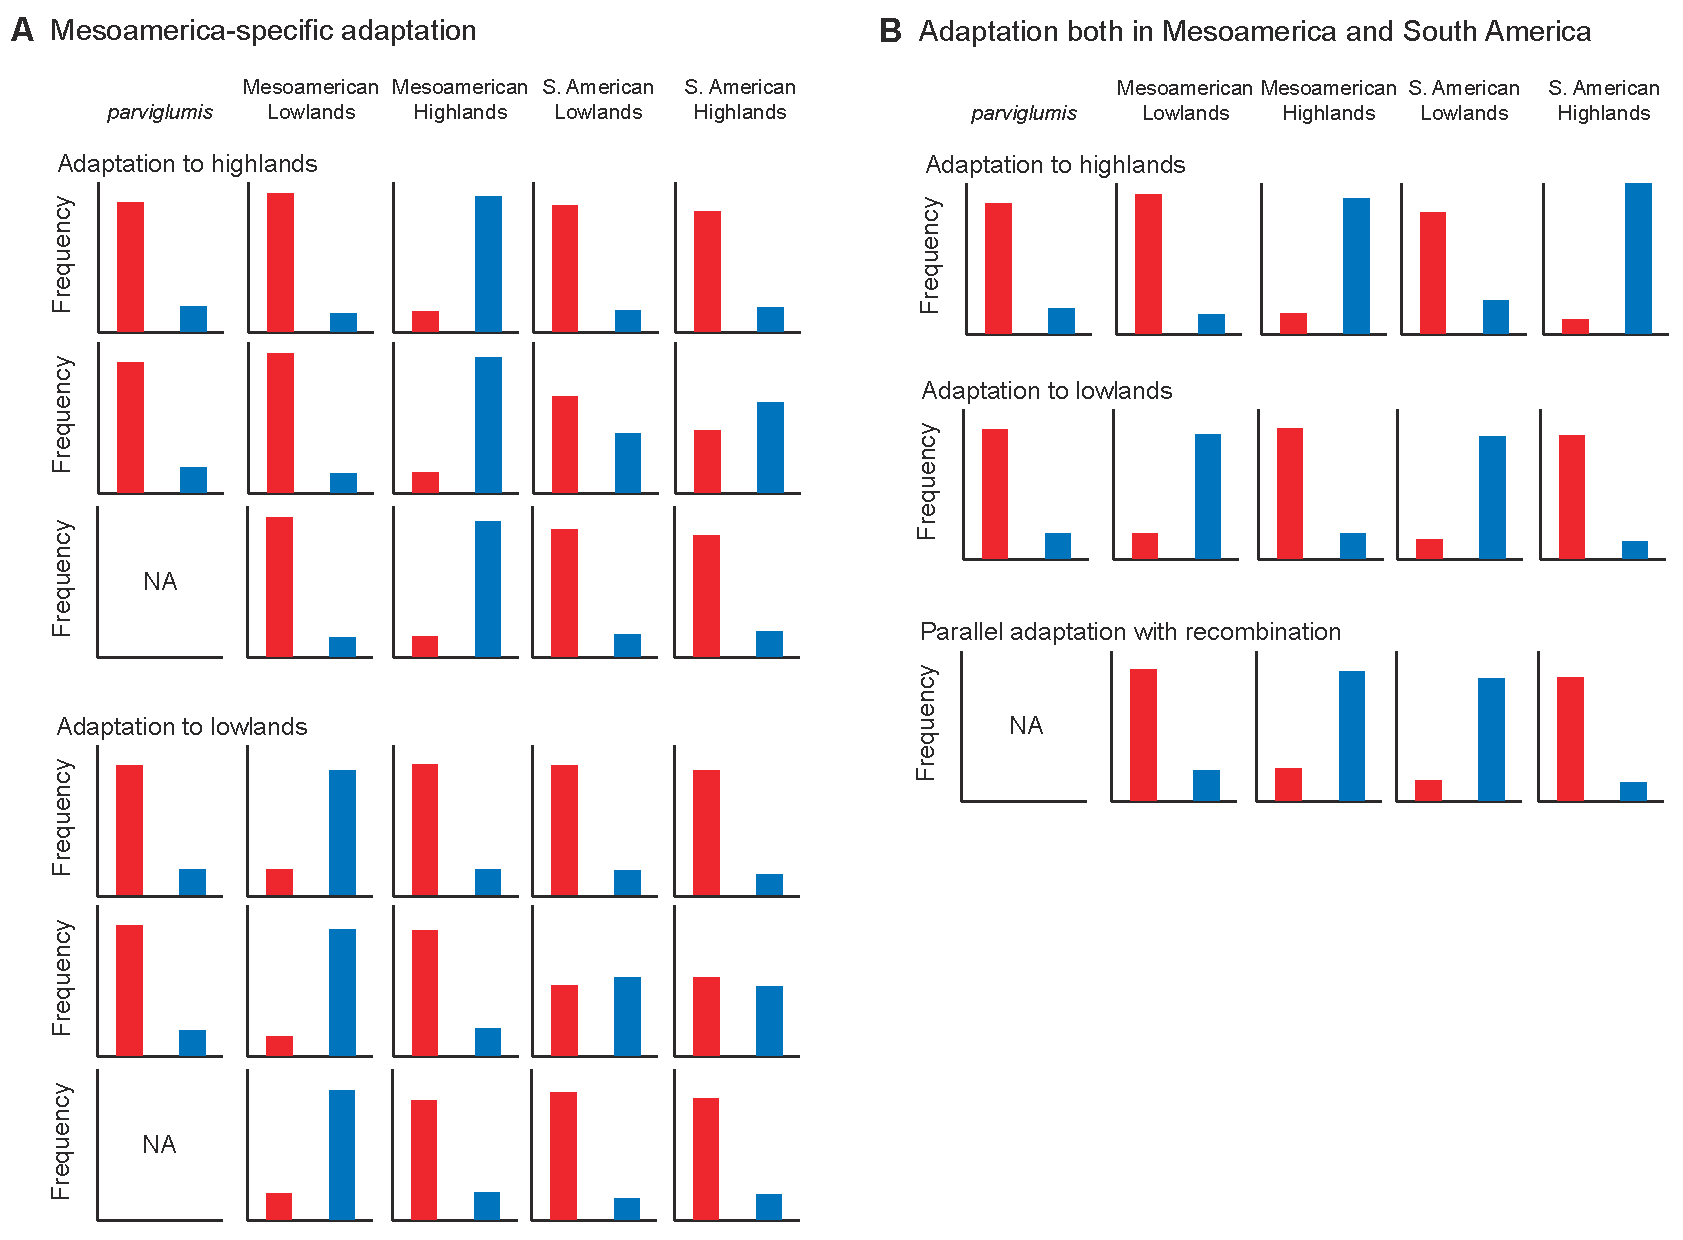
\includegraphics[width=0.9\columnwidth]{fig/AllelePat.pdf}
    \caption{Illustration of allele frequency changes in maize and \emph{parviglumis}.  Red and blue bars represent the allele frequency of ancestral and derived, adaptive alleles, respectively.  The allele frequencies in the five populations are shown: \emph{parviglumis}, Mexican lowlands and highlands, and S. America lowlands and highlands. NA in \emph{parviglumis} indicates that there is no SNP data in the site.}
    \label{AllelePat}
  \end{center}
\end{figure}
%%%%%%%%%%%%%%%%%%%%%%%%%%%%%%%%%%%%%%%%%%%%%%%%%%%%%%%%%%%%

\clearpage
\suppl

%\section*{SUPPLEMENTAL METHODS}
\renewcommand{\thefigure}{S\arabic{figure}}
\renewcommand{\thetable}{S\arabic{table}}


%%%%%%%%%%%%%%%%%%%%%%%%%%%%%%%
%Table S1 %
\renewcommand{\arraystretch}{1.2}

\begin{table}[h]
    \begin{center}
    \caption[]{List of maize landraces used in this study\hspace*{7.5cm}}  
{\fontsize{7}{10}\selectfont
%{\small
    \begin{tabular}{llllllllll}
        \hline\hline
       & & & \\[-4mm] 
	 ID$^a$	&	USDA ID	&	Population	&	Landrace	&	Locality	&	Latitude	&	Longitude	&	Elevation	&	Origin	\\[0.0cm]
	\hline 
	& & & \\[-4mm] 
{\bf RIMMA0409}	&	PI 478968	&	Mexico 	&	Tepecintle	&	Chiapas, Mexico	&	15.4 	&	-92.9 	&	107	&	USDA	\\
RIMMA0410	&	PI 478970	&	Lowland	&	Vandeno	&	Chiapas, Mexico	&	15.4 	&	-92.9 	&	107	&	USDA	\\
{\bf RIMMA0433}	&	PI 490825	&		&	Nal Tel ATB	&	Chiquimula, Guatemala	&	14.7 	&	-89.5 	&	457	&	USDA	\\
{\bf RIMMA0441}	&	PI 515538	&		&	Coscomatepec	&	Veracruz, Mexico	&	19.2 	&	-97.0 	&	1320	&	USDA	\\
{\bf RIMMA0615}	&	PI 628480	&		&	Tuxpeno	&	Puebla, Mexico	&	20.1 	&	-97.2 	&	152	&	USDA	\\
{\bf RIMMA0619}	&	PI 645772	&		&	Pepitilla	&	Guerrero, Mexico	&	18.4 	&	-99.5 	&	747	&	USDA	\\
{\bf RIMMA0628}	&	PI 646017	&		&	Tuxpeno Norteno	&	Tamaulipas, Mexico	&	23.3 	&	-99.0 	&	300	&	USDA	\\
{\bf RIMMA0696}	&	Ames 28568	&		&	Tuxpeno	&	El Progreso, Guatemala	&	16.5 	&	-90.2 	&	30	&	Goodman	\\
{\bf RIMMA0700}	&	NSL 291626	&		&	Olotillo	&	Chiapas, Mexico	&	16.8 	&	-93.2 	&	579	&	Goodman	\\
{\bf RIMMA0701}	&	PI 484808	&		&	Olotillo	&	Chiapas, Mexico	&	16.6 	&	-92.7 	&	686	&	Goodman	\\
{\bf RIMMA0702}	&	Ames 28534	&		&	Negro de Tierra Caliente	&	Sacatepequez, Guatemala	&	14.5 	&	-90.8 	&	1052	&	Goodman	\\
{\bf RIMMA0703}	&	NSL 283390	&		&	Nal Tel	&	Yucatan, Mexico	&	20.8 	&	-88.5 	&	30	&	Goodman	\\
{\bf RIMMA0709}	&	Ames 28452	&		&	Tehua	&	Chiapas, Mexico	&	16.5 	&	-92.5 	&	747	&	Goodman	\\
{\bf RIMMA0710}	&	PI 478988	&		&	Tepecintle	&	Chiapas, Mexico	&	15.3 	&	-92.6 	&	91	&	Goodman	\\
{\bf RIMMA0712}	&	NSL 291696 CYMT	&		&	Oloton	&	Baja Verapaz, Guatemala	&	15.3 	&	-90.3 	&	1220	&	Goodman	\\
{\bf RIMMA0716}	&	Ames 28459	&		&	Zapalote Grande	&	Chiapas, Mexico	&	15.3 	&	-92.7 	&	91	&	Goodman	\\
{\bf RIMMA0720}	&	PI 489372	&		&	Negro de Tierra Caliente	&	Guatemala	&	15.5 	&	-88.9 	&	39	&	Goodman	\\
{\bf RIMMA0721}	&	Ames 28485	&		&	Nal Tel ATB	&	Chiquimula, Guatemala	&	14.6 	&	-90.1 	&	915	&	Goodman	\\
{\bf RIMMA0722}	&	Ames 28564	&		&	Dzit Bacal	&	Jutiapa, Guatemala	&	14.3 	&	-89.7 	&	737	&	Goodman	\\
{\bf RIMMA0727}	&	Ames 28555	&		&	Comiteco	&	Guatemala	&	14.4 	&	-90.5 	&	1151	&	Goodman	\\
{\bf RIMMA0729}	&	PI 504090	&		&	Tepecintle	&	Guatemala	&	15.4 	&	-89.7 	&	122	&	Goodman	\\
{\bf RIMMA0730}	&	Ames 28517	&		&	Quicheno Late	&	Sacatepequez, Guatemala	&	14.5 	&	-90.8 	&	1067	&	Goodman	\\
{\bf RIMMA0731}	&	PI 484137	&		&	Bolita	&	Oaxaca, Mexico	&	16.8 	&	-96.7 	&	1520	&	Goodman	\\
{\bf RIMMA0733}	&	PI 479054	&		&	Zapalote Chico	&	Oaxaca, Mexico	&	16.6 	&	-94.6 	&	107	&	Goodman	\\
	\hline 
	& & & \\[-4mm] 
{\bf RIMMA0416}	&	PI 484428	&	Mexico	&	Cristalino de Chihuahua	&	Chihuahua, Mexico	&	29.4 	&	-107.8 	&	2140	&	NA	\\
{\bf RIMMA0417}	&	PI 484431	&	Highland	&	Azul	&	Chihuahua, Mexico	&	28.6 	&	-107.5 	&	2040	&	USDA	\\
{\bf RIMMA0418}	&	PI 484476	&		&	Gordo	&	Chihuahua, Mexico	&	28.6 	&	-107.5 	&	2040	&	USDA	\\
{\bf RIMMA0421}	&	PI 484595	&		&	Conico	&	Puebla, Mexico	&	19.9 	&	-98.0 	&	2250	&	USDA	\\
{\bf RIMMA0422}	&	PI 485071	&		&	Elotes Conicos	&	Puebla, Mexico	&	19.1 	&	-98.3 	&	2200	&	USDA	\\
{\bf RIMMA0423}	&	PI 485116	&		&	Cristalino de Chihuahua	&	Chihuahua, Mexico	&	29.2 	&	-108.1 	&	2095	&	NA	\\
{\bf RIMMA0424}	&	PI 485120	&		&	Apachito	&	Chihuahua, Mexico	&	28.0 	&	-107.6 	&	2400	&	USDA	\\
{\bf RIMMA0425}	&	PI 485128	&		&	Palomero Tipo Chihuahua	&	Chihuahua, Mexico	&	26.8 	&	-107.1 	&	2130	&	USDA	\\
{\bf RIMMA0614}	&	PI 628445	&		&	Mountain Yellow	&	Jalisco, Mexico	&	20.0 	&	-103.8 	&	2060	&	USDA	\\
{\bf RIMMA0616}	&	PI 629202	&		&	Zamorano Amarillo	&	Jalisco, Mexico	&	20.8 	&	-102.8 	&	1800	&	USDA	\\
{\bf RIMMA0620}	&	PI 645786	&		&	Celaya	&	Guanajuato, Mexico	&	20.2 	&	-100.9 	&	1799	&	USDA	\\
{\bf RIMMA0621}	&	PI 645804	&		&	Zamorano Amarillo	&	Guanajuato, Mexico	&	21.1 	&	-101.7 	&	1870	&	USDA	\\
{\bf RIMMA0623}	&	PI 645841	&		&	Palomero de Jalisco	&	Jalisco, Mexico	&	20.0 	&	-103.7 	&	2520	&	USDA	\\
{\bf RIMMA0625}	&	PI 645984	&		&	Cacahuacintle	&	Puebla, Mexico	&	19.0 	&	-97.4 	&	2600	&	USDA	\\
RIMMA0626	&	PI 645993	&		&	Arrocillo Amarillo	&	Puebla, Mexico	&	19.9 	&	-97.6 	&	2260	&	USDA	\\
{\bf RIMMA0630}	&	PI 646069	&		&	Arrocillo Amarillo	&	Veracruz, Mexico	&	19.8 	&	-97.3 	&	2220	&	USDA	\\
{\bf RIMMA0670}	&	Ames 28508	&		&	San Marceno	&	San Marcos, Guatemala	&	15.0 	&	-91.8 	&	2378	&	Goodman	\\
{\bf RIMMA0671}	&	Ames 28538	&		&	Salpor Tardio	&	Solola, Guatemala	&	14.8 	&	-91.3 	&	2477	&	Goodman	\\
{\bf RIMMA0672}	&	PI 483613	&		&	Chalqueno	&	Mexico, Mexico	&	19.7 	&	-99.1 	&	2256	&	Goodman	\\
{\bf RIMMA0674}	&	PI 483617	&		&	Toluca	&	Mexico, Mexico	&	19.3 	&	-99.7 	&	2652	&	Goodman	\\
{\bf RIMMA0677}	&	Ames 28476 	&		&	Conico Norteno	&	Zacatecas, Mexico	&	21.4 	&	-102.9 	&	1951	&	Goodman	\\
{\bf RIMMA0680}	&	Ames 28448	&		&	Tabloncillo	&	Jalisco, Mexico	&	20.4 	&	-102.2 	&	1890	&	Goodman	\\
{\bf RIMMA0682}	&	PI 484571	&		&	Tablilla de Ocho	&	Jalisco, Mexico	&	22.1 	&	-103.2 	&	1700	&	Goodman	\\
{\bf RIMMA0687}	&	Ames 28473	&		&	Conico Norteno	&	Queretaro, Mexico	&	20.4 	&	-100.0 	&	1921	&	Goodman	\\[-0.1mm]	
	                         %&                       &                                 & \emph{BoS-68}  & AB298905       &  AB054737\\[-0.1mm]	
	\hline\hline
\multicolumn{9}{l}{$^a$ GBS data are available for the accessions in bold font.}\\
    \end{tabular}}
    \label{srkid}

\end{center} 

\end{table}

\clearpage
%%%%%%%%%%%%%%%%%%%%%%%%%%%%%%%%%%%%%%%%%%%

\setcounter{table}{0}
%%%%%%%%%%%%%%%%%%%%%%%%%%%%%%%
%Table S1 %
\renewcommand{\arraystretch}{1.2}

\begin{table}[h]
    \begin{center}
    \caption[]{(continued)\hspace*{11.8cm}}  
{\fontsize{7}{10}\selectfont
%{\small
    \begin{tabular}{llllllllll}
        \hline\hline
       & & & \\[-4mm] 
	 ID	&	USDA ID	&	Population	&	Landrace	&	Locality	&	Latitude	&	Longitude	&	Elevation	&	Origin	\\[0.0cm]
	\hline 
	& & & \\[-4mm] 
{\bf RIMMA0388}	&	PI 443820	&	South America	&	Amagaceno	&	Antioquia, Colombia	&	6.9 	&	-75.3 	&	1500	&	USDA	\\
{\bf RIMMA0389}	&	PI 444005	&	Lowland	&	Costeno	&	Atlantico, Colombia	&	10.4 	&	-74.9 	&	7	&	USDA	\\
{\bf RIMMA0390}	&	PI 444254	&		&	Comun	&	Caldas, Colombia	&	4.5 	&	-75.6 	&	353	&	USDA	\\
RIMMA0391	&	PI 444296	&		&	Andaqui	&	Caqueta, Colombia	&	1.4 	&	-75.8 	&	700	&	USDA	\\
{\bf RIMMA0392}	&	PI 444309	&		&	Andaqui	&	Caqueta, Colombia	&	1.8 	&	-75.6 	&	555	&	USDA	\\
{\bf RIMMA0393}	&	PI 444473	&		&	Costeno	&	Cordoba, Colombia	&	8.3 	&	-75.2 	&	100	&	USDA	\\
{\bf RIMMA0394}	&	PI 444621	&		&	Pira	&	Cundinamarca, Colombia	&	4.8 	&	-74.7 	&	1000	&	USDA	\\
{\bf RIMMA0395}	&	PI 444731	&		&	Negrito	&	Choco, Colombia	&	8.5 	&	-77.3 	&	30	&	USDA	\\
{\bf RIMMA0396}	&	PI 444834	&		&	Caqueteno	&	Huila, Colombia	&	2.6 	&	-75.3 	&	1100	&	USDA	\\
{\bf RIMMA0397}	&	PI 444897	&		&	Negrito	&	Magdalena, Colombia	&	11.6 	&	-72.9 	&	50	&	USDA	\\
{\bf RIMMA0398}	&	PI 444923	&		&	Puya	&	Magdalena, Colombia	&	9.4 	&	-75.7 	&	27	&	USDA	\\
{\bf RIMMA0399}	&	PI 444954	&		&	Cariaco	&	Magdalena, Colombia	&	10.2 	&	-74.1 	&	250	&	USDA	\\
{\bf RIMMA0403}	&	PI 445163	&		&	Pira Naranja	&	Narino, Colombia	&	1.3 	&	-77.5 	&	1000	&	USDA	\\
{\bf RIMMA0404}	&	PI 445322	&		&	Puya Grande	&	Norte de Santander, Colombia	&	7.3 	&	-72.5 	&	1500	&	USDA	\\
RIMMA0405	&	PI 445355	&		&	Puya	&	Norte de Santander, Colombia	&	8.4 	&	-73.3 	&	1100	&	USDA	\\
{\bf RIMMA0406}	&	PI 445514	&		&	Yucatan	&	Tolima, Colombia	&	5.0 	&	-74.9 	&	450	&	USDA	\\
RIMMA0407	&	PI 445528	&		&	Pira	&	Tolima, Colombia	&	4.2 	&	-74.9 	&	450	&	USDA	\\
{\bf RIMMA0428}	&	PI 485354	&		&	Aleman	&	Huanuco, Peru	&	-9.3 	&	-76.0 	&	700	&	NA	\\
{\bf RIMMA0462}	&	PI 445073	&		&	Amagaceno	&	Narino, Colombia	&	1.6 	&	-77.2 	&	1700	&	USDA	\\
{\bf RIMMA0690}	&	PI 444946	&		&	Puya	&	Magdalena, Colombia	&	8.3 	&	-73.6 	&	250	&	Goodman	\\
{\bf RIMMA0691}	&	PI 445391	&		&	Cacao	&	Santander, Colombia	&	6.6 	&	-73.1 	&	1098	&	NA	\\
{\bf RIMMA0707}	&	PI 487930	&		&	Tuxpeno	&	Ecuador	&	-1.1 	&	-80.5 	&	30	&	Goodman	\\
{\bf RIMMA0708}	&	PI 488376	&		&	Yunquillano F Andaqui	&	Ecuador	&	-3.5 	&	-78.6 	&	1098	&	Goodman	\\
	\hline 
	& & & \\[-4mm] 
{\bf RIMMA0426}	&	PI 485151	&	South America	&	Rabo de Zorro	&	Ancash, Peru	&	-9.1 	&	-77.8 	&	2500	&	NA	\\
{\bf RIMMA0430}	&	PI 485362	&	Highland	&	Sarco	&	Ancash, Peru	&	-9.2 	&	-77.7 	&	2585	&	NA	\\
{\bf RIMMA0431}	&	PI 485363	&	(Andean)	&	Perlilla	&	Huanuco, Peru	&	-8.7 	&	-77.1 	&	2900	&	NA	\\
{\bf RIMMA0436}	&	PI 514723	&		&	Morocho Cajabambino	&	Amazonas, Peru	&	-6.2 	&	-77.9 	&	2200	&	NA	\\
{\bf RIMMA0437}	&	PI 514752	&		&	Ancashino	&	Ancash, Peru	&	-9.3 	&	-77.6 	&	2688	&	NA	\\
{\bf RIMMA0438}	&	PI 514809	&		&	Maranon	&	Ancash, Peru	&	-8.7 	&	-77.4 	&	2820	&	NA	\\
RIMMA0439	&	PI 514969	&		&	Maranon	&	La Libertad, Peru	&	-8.5 	&	-77.2 	&	2900	&	NA	\\
{\bf RIMMA0464}	&	PI 571438	&		&	Chullpi	&	Huancavelica, Peru	&	-12.3 	&	-74.7 	&	1800	&	USDA	\\
{\bf RIMMA0465}	&	PI 571457	&		&	Huarmaca	&	Piura, Peru	&	-5.6 	&	-79.5 	&	2300	&	USDA	\\
{\bf RIMMA0466}	&	PI 571577	&		&	Confite Puneno	&	Apurimac, Peru	&	-14.3 	&	-72.9 	&	3600	&	USDA	\\
{\bf RIMMA0467}	&	PI 571871	&		&	Paro	&	Apurimac, Peru	&	-13.6 	&	-72.9 	&	2800	&	USDA	\\
{\bf RIMMA0468}	&	PI 571960	&		&	Sarco	&	Ancash, Peru	&	-9.4 	&	-77.2 	&	3150	&	USDA	\\
{\bf RIMMA0473}	&	PI 445114	&		&	Sabanero	&	Narino, Colombia	&	1.1 	&	-77.6 	&	3104	&	USDA	\\
{\bf RIMMA0656}	&	Ames 28799	&		&	Culli	&	Jujuy, Argentina	&	-23.2 	&	-65.4 	&	2287	&	Goodman	\\
{\bf RIMMA0657}	&	NSL 286594	&		&	Chake Sara	&	Bolivia	&	-17.5 	&	-65.7 	&	2201	&	Goodman	\\
{\bf RIMMA0658}	&	NSL 286812	&		&	Uchuquilla	&	Bolivia	&	-21.8 	&	-64.1 	&	1948	&	Goodman	\\
{\bf RIMMA0661}	&	PI 488066	&		&	Chillo	&	Ecuador	&	-2.9 	&	-78.7 	&	2195	&	Goodman	\\
{\bf RIMMA0662}	&	NSL 287008	&		&	Cuzco	&	Ecuador	&	0.0 	&	-78.0 	&	2195	&	Goodman	\\
{\bf RIMMA0663}	&	PI 488102	&		&	Mishca	&	Ecuador	&	0.4 	&	-78.2 	&	2067	&	Goodman	\\
{\bf RIMMA0664}	&	PI 488113	&		&	Blanco Blandito	&	Ecuador	&	0.4 	&	-78.4 	&	2122	&	Goodman	\\
{\bf RIMMA0665}	&	PI 489324	&		&	Racimo de Uva	&	Ecuador	&	-0.9 	&	-78.9 	&	2931	&	Goodman	\\
{\bf RIMMA0667}	&	Ames 28737	&		&	Patillo	&	Chuquisaca, Bolivia	&	-21.8 	&	-64.1 	&	2201	&	NA	\\
RIMMA0668	&	Ames 28668	&		&	Granada	&	Puno, Peru	&	-14.9 	&	-70.6 	&	3925	&	Goodman	\\[-0.1mm] 
	                         %&                       &                                 & \emph{BoS-68}  & AB298905       &  AB054737\\[-0.1mm]	
	\hline\hline
	\multicolumn{9}{l}{$^a$ GBS data are available for the accessions in bold font.}\\
    \end{tabular}}
    \label{srkid}

\end{center} 

\end{table}

\clearpage
%%%%%%%%%%%%%%%%%%%%%%%%%%%%%%%%%%%%%%%%%%%




%%%%%%%%%%%%%%%%%%%%%%%%%%%%%%%%%%%%%%%%%%%%%%%%%%%%%%%%%%%%
\renewcommand{\arraystretch}{1.1}
\begin{table}[tb]

\begin{center}
 \caption[]{Inference of demographic parameters\hspace*{0.3cm}}
  \textbf{}\\[-2mm]
{\fontsize{8}{11}\sf
    \begin{tabular}{ccccccccl} \hline
       & & \\[-3mm]
     Mexico  & \multicolumn{2}{c}{Model I}  \\[0.1cm]
    \hline
    & & \\[-3mm]
   & Likelihood & $-$3052.34  \\
  &$\alpha$ & 0.99 \\
  &$\beta$ & 0.42 \\ 
  &$\gamma$   & 1        \\ 
  & $\sigma$ & 1\\
      \hline
    & & \\[-3mm]
    South America  & \multicolumn{2}{c}{Model I}  \\[0.1cm]
        \hline
    & & \\[-3mm]
     & Likelihood &  $-$2717.64  \\
       &$\alpha$ & 0.51 \\
      &$\beta$ & 0.97           \\ 
      &$\gamma$   & 151   \\
        & $\sigma$ & 1\\ [1mm]
    \hline
\multicolumn{3}{l}{The description of $\alpha, \beta$ and $\gamma$ is in Figure~3.}\\
\multicolumn{3}{l}{$\sigma$ is a relative size of $N_B$ to $N_C$ ($N_B=\sigma N_C$).}\\
    \end{tabular}
    \label{supp:param}  % caption is needed to make this work
}
\end{center}
\end{table}
\renewcommand{\arraystretch}{1}
%%%%%%%%%%%%%%%%%%%%%%%%%%%%%%%%%%%%%%%%%%%%%%%%%%%%%%%%%%%%


%%%%%%%%%%%%%%%%%%%%%%%%%%%%%%%%%%%%%%%%%%%%%%%%%%%%%%%%%%%%
\renewcommand{\arraystretch}{1.1}
\begin{table}[tb]

\begin{center}
 \caption[]{Summary of PHS test\hspace*{5.3cm}}
  \textbf{}\\[-2mm]
{\fontsize{8}{11}\sf
    \begin{tabular}{lllllcccccl} \hline
       & & \\[-3mm]
     Population  & Pattern of adaptation & No. SNPs & No. SNPs supported by PHS test \\[0.1cm]
    \hline
    & & \\[-3mm]
   Mexico & Highland adaptation & 264 & 172 (65.2\%)  \\
               & Lowland adaptation & 101 & 66 (65.3\%)  \\
   S. America & Highland adaptation & 164 & 230 (71.3\%)  \\
                     & Lowland adaptation & 70 & 50 (71.4\%)  \\[0.1cm]
    \hline
    \end{tabular}
    \label{supp:phs}  % caption is needed to make this work
}
\end{center}
\end{table}
\renewcommand{\arraystretch}{1}
%%%%%%%%%%%%%%%%%%%%%%%%%%%%%%%%%%%%%%%%%%%%%%%%%%%%%%%%%%%%



%%%%%%%%%%%%%%%%%%%%%%%%%%%%%%%%%%%%%%%%%%%%%%%%%%%%%%%%%%%%
\renewcommand{\arraystretch}{1.1}
\begin{table}[tb]

\begin{center}
 \caption[]{ms command\hspace*{11.3cm}}
  \textbf{}\\[-2mm]
{\fontsize{7}{11}\sf
    \begin{tabular}{llcccccccl} \hline
       & & \\[-3mm]
     Model I for Mexico  populations   \\
     Population 1: Mexico lowland population   \\
     Population 2: Mexico highland population   \\
  -I 2 $n_{m1}$ $n_{m2}$ -n 1 0.3496 -n 2 0.5704 -ej 0.01 2 1 -en 0.01 1 0.92 -en 0.0133 1 0.0163 -en 0.015 1 1.0 \\ 
      \hline
    & & \\[-3mm]
     Model II for Mexico  populations   \\
     Population 1: Mexico lowland population   \\
     Population 2: Mexico highland population   \\
     Population 3: \emph{mexicane} population   \\
-I 2 $n_{m1}$ $n_{m2}$ -n 1 1.14 -n 2 0.36 -es 0.01 2 0.8 -en 0.01 3 1.0667 -ej 0.01 2 1 -en 0.01 1 1.5 -en 0.0133 1 0.0163 -en 0.015 1 1.0 -ej 0.1 3 1 \\ 
      \hline
    & & \\[-3mm]
    Model I for SA  populations   \\
     Population 1: SA lowland population   \\
     Population 2: SA highland population   \\
  -I 2 $n_{s1}$ $n_{s2}$ -n 1 0.5044 -n 2 1.3728 -g 2 671.60 -ej 0.006667 2 1 -eg 0.006667 2 0.0 -en 0.00667 1 0.52 -en 0.01333 1 0.0163 -en 0.015 1 1.0 \\ 
      \hline
    & & \\[-3mm]
    Model III for SA  populations   \\
    Population 1: Mexico lowland population   \\
     Population 2: SA lowland population   \\
     Population 3: SA highland population   \\
  -I 3 $n_{m1}$ $n_{s1}$ $n_{s2}$ -n 1 0.64 -n 2 0.342 -n 3 0.972 -g 3 598.35 -ej 0.006667 3 2 -eg 0.006667 3 0.0 -en 0.006667 2 0.36 -ej 0.01 2 1\\
   -en 0.01 1 1 -en 0.0133 1 0.0163 -en 0.015 1 1.0 \\  [1mm]
    \hline
\multicolumn{1}{l}{Sample size of Mexico lowland, Mexico highland, SA lowland and SA highland populations are denoted by $n_{m1}$, $n_{m2}$, $n_{s1}$ and $n_{s2}$, respectively.}\\
    \end{tabular}
    \label{commandline}  % caption is needed to make this work
}
\end{center}
\end{table}
\renewcommand{\arraystretch}{1}
%%%%%%%%%%%%%%%%%%%%%%%%%%%%%%%%%%%%%%%%%%%%%%%%%%%%%%%%%%%%

%%%%%%%%%%%%%%%%%%%%%%%%%%%%%%%%%%%%%%%%%%%%%%%%%%%%%%%%%%%%
\begin{figure}[t]
  \begin{center}
    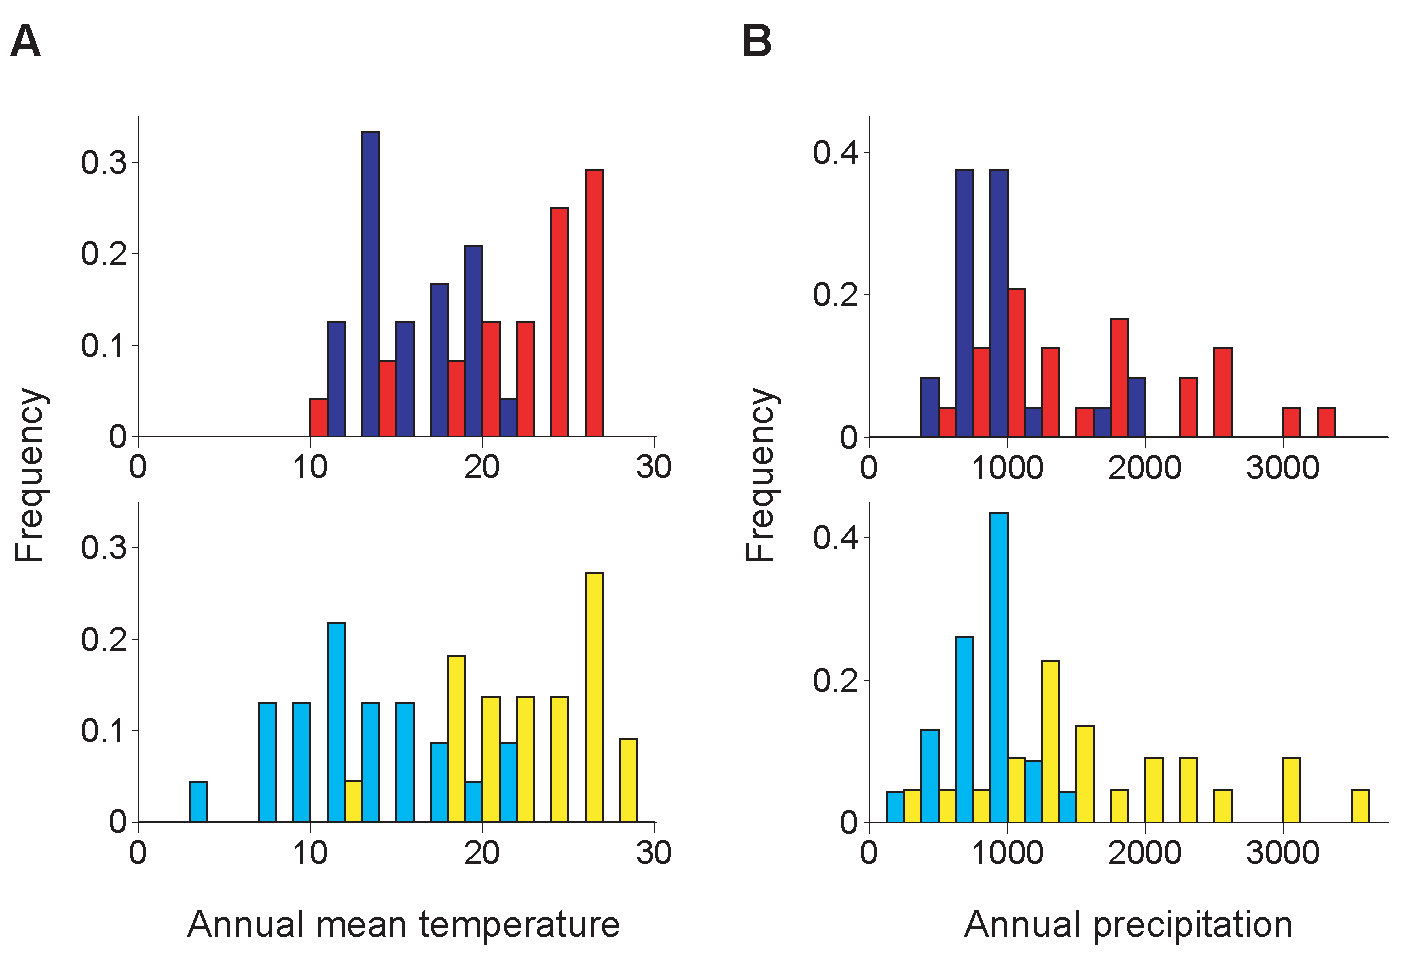
\includegraphics[width=0.6\columnwidth]{fig/bioclm.pdf}
    \caption{Correlation of allele frequencies between GBS (\emph{x}-axes) and MaizeSNP50 (\emph{y}-axes) data.  We used overlapped SNPs with $n\geq40$ for both data sets.  Correlation coefficient is 0.890 ($P<10^{-5}$ by permutation test with $10^5$ replications).}
    \label{supp:colfreq}
  \end{center}
\end{figure}
%%%%%%%%%%%%%%%%%%%%%%%%%%%%%%%%%%%%%%%%%%%%%%%%%%%%%%%%%%%%

%%%%%%%%%%%%%%%%%%%%%%%%%%%%%%%%%%%%%%%%%%%%%%%%%%%%%%%%%%%%
\begin{figure}[t]
  \begin{center}
    \includegraphics[width=0.4\columnwidth]{fig/col.pdf}
    \caption{Correlation of allele frequencies between GBS (\emph{x}-axes) and MaizeSNP50 (\emph{y}-axes) data.  We used overlapped SNPs with $n\geq40$ for both data sets.  Correlation coefficient is 0.890 ($P<10^{-5}$ by permutation test with $10^5$ replications).}
    \label{supp:correl_freq}
  \end{center}
\end{figure}
%%%%%%%%%%%%%%%%%%%%%%%%%%%%%%%%%%%%%%%%%%%%%%%%%%%%%%%%%%%%

%%%%%%%%%%%%%%%%%%%%%%%%%%%%%%%%%%%%%%%%%%%%%%%%%%%%%%%%%%%%
\begin{figure}[t]
  \begin{center}
    \includegraphics[width=0.4\columnwidth]{fig/kk.pdf}
    \caption{Likelihood of STRUCTURE analysis given $K$.  The \emph{x}-axes represents $K$ and the \emph{y}-axes represents likelihood.}
    \label{supp:struct}
  \end{center}
\end{figure}
%%%%%%%%%%%%%%%%%%%%%%%%%%%%%%%%%%%%%%%%%%%%%%%%%%%%%%%%%%%%

%%%%%%%%%%%%%%%%%%%%%%%%%%%%%%%%%%%%%%%%%%%%%%%%%%%%%%%%%%%%
\begin{figure}[t]
  \begin{center}
    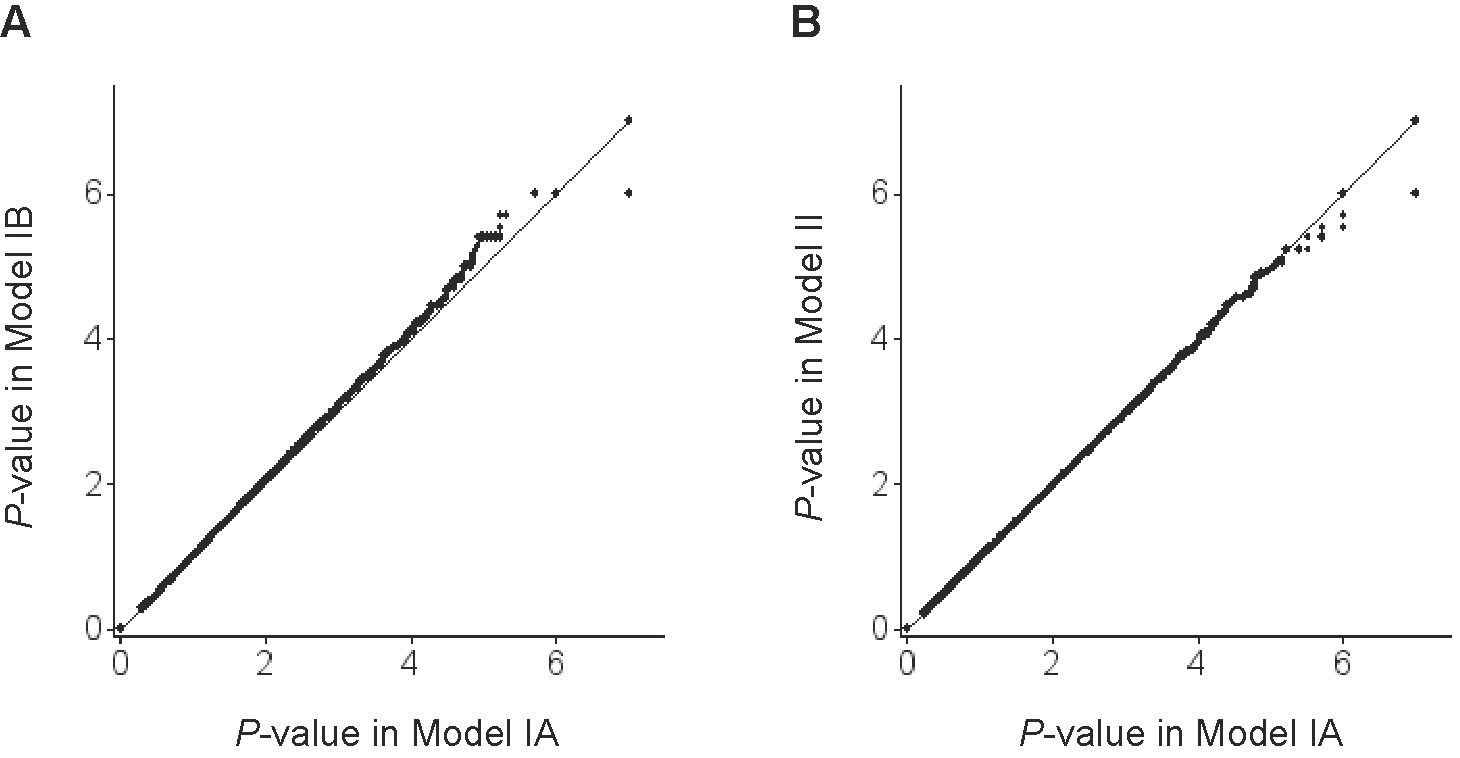
\includegraphics[width=0.6\columnwidth]{fig/bot2.pdf}
    \caption{Q-Q plot for $-$log$_{10}$-scaled \emph{P}-values of population differentiation between lowland and highland populations. (A) Model IA \emph{v.s.} Model IB in Mexico, (B) Model IA \emph{v.s.} Model II in S. America, (C) Model with \emph{v.s.} without bottleneck in Mexico and (D) Model with \emph{v.s.} without bottleneck in S. America.}
    \label{fig:qq}
  \end{center}
\end{figure}
%%%%%%%%%%%%%%%%%%%%%%%%%%%%%%%%%%%%%%%%%%%%%%%%%%%%%%%%%%%%


%%%%%%%%%%%%%%%%%%%%%%%%%%%%%%%%%%%%%%%%%%%%%%%%%%%%%%%%%%%%
%\begin{figure}[t]
%  \begin{center}
%    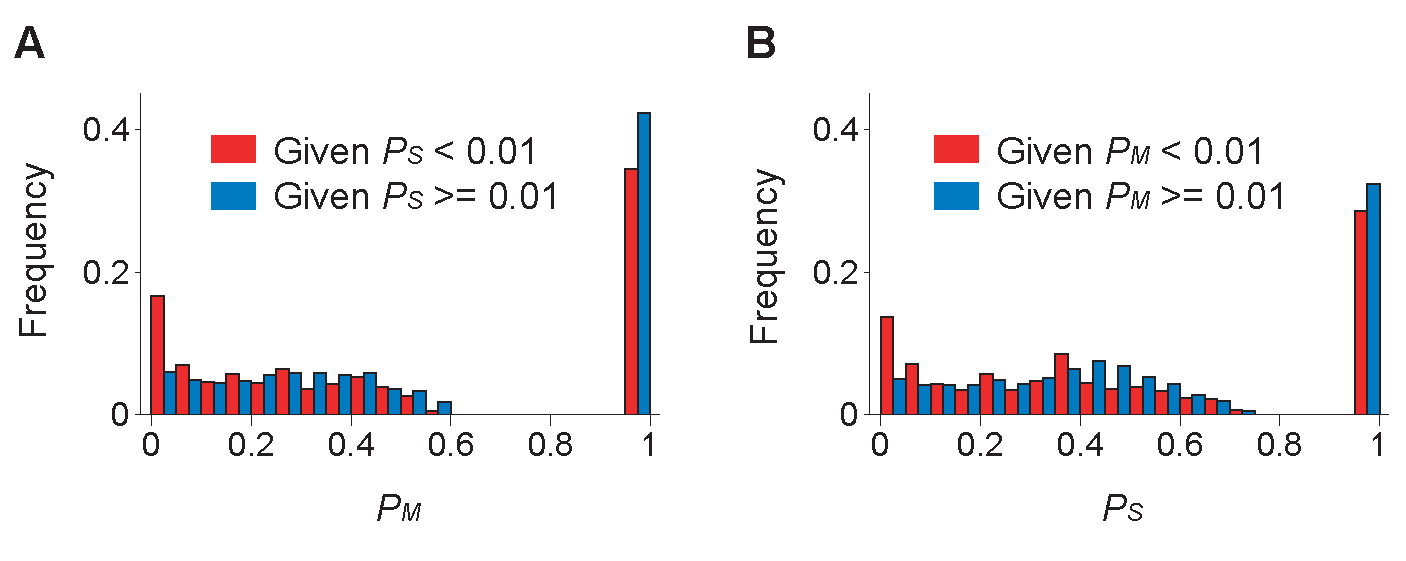
\includegraphics[width=0.8\columnwidth]{fig/pmps.pdf}
%    \caption{(A) Frequency distribution of $P_M$ given $P_S<0.01$ and $P_S\geq0.01$.  (B) Frequency distribution of $P_S$ given $P_M<0.01$ and $P_M\geq0.01$.}
%    \label{pval_freq_comparison}
%  \end{center}
%\end{figure}
%%%%%%%%%%%%%%%%%%%%%%%%%%%%%%%%%%%%%%%%%%%%%%%%%%%%%%%%%%%%

%%%%%%%%%%%%%%%%%%%%%%%%%%%%%%%%%%%%%%%%%%%%%%%%%%%%%%%%%%%%
\begin{figure}[t]
  \begin{center}
    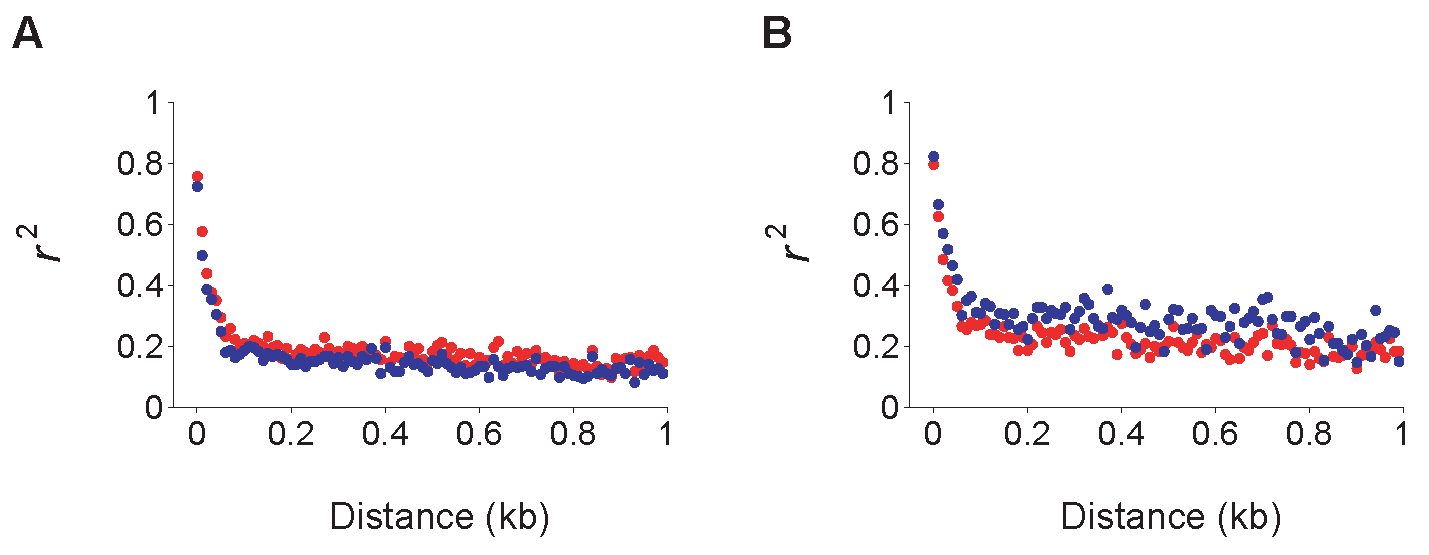
\includegraphics[width=0.7\columnwidth]{fig/LD.pdf}
    \caption{Pattern of decay of linkage equilibrium in Mexico (A) and South America (B).  Red and blue dots represent low- and highland population, respectively.  $r^2$ values were calculated as a statistics and averaged within 10-bp bins of distance between SNPs.  The \emph{x}- and \emph{y}-axes represent distance between SNPs (kb) and average $r^2$ values.}
    \label{supp:LD}
  \end{center}
\end{figure}
%%%%%%%%%%%%%%%%%%%%%%%%%%%%%%%%%%%%%%%%%%%%%%%%%%%%%%%%%%%%








%%%%%%%%%%%%%%%%%%%%%%%%%%%%%%%%%%%%%%%%%%%%%%%%%%%%%%%%%%%%
%\begin{figure}[t]
%  \begin{center}
%    \includegraphics[width=0.6\columnwidth]{fig/GBSP.pdf}
%    \caption{Q-Q plot for $-$log$_{10}$-scaled \emph{P}-values of population differentiation between models in GBS data. The results of Mexico (A) and South America (B) are shown. The solid lines represent \emph{y}=\emph{x}.}
%    \label{colfreq}
%  \end{center}
%\end{figure}
%%%%%%%%%%%%%%%%%%%%%%%%%%%%%%%%%%%%%%%%%%%%%%%%%%%%%%%%%%%%



%%%%%%%%%%%%%%%%%%%%%%%%%%%%%%%%%%%%%%%%%%%%%%%%%%%%%%%%%%%%
%\begin{figure}[t]
%  \begin{center}
%    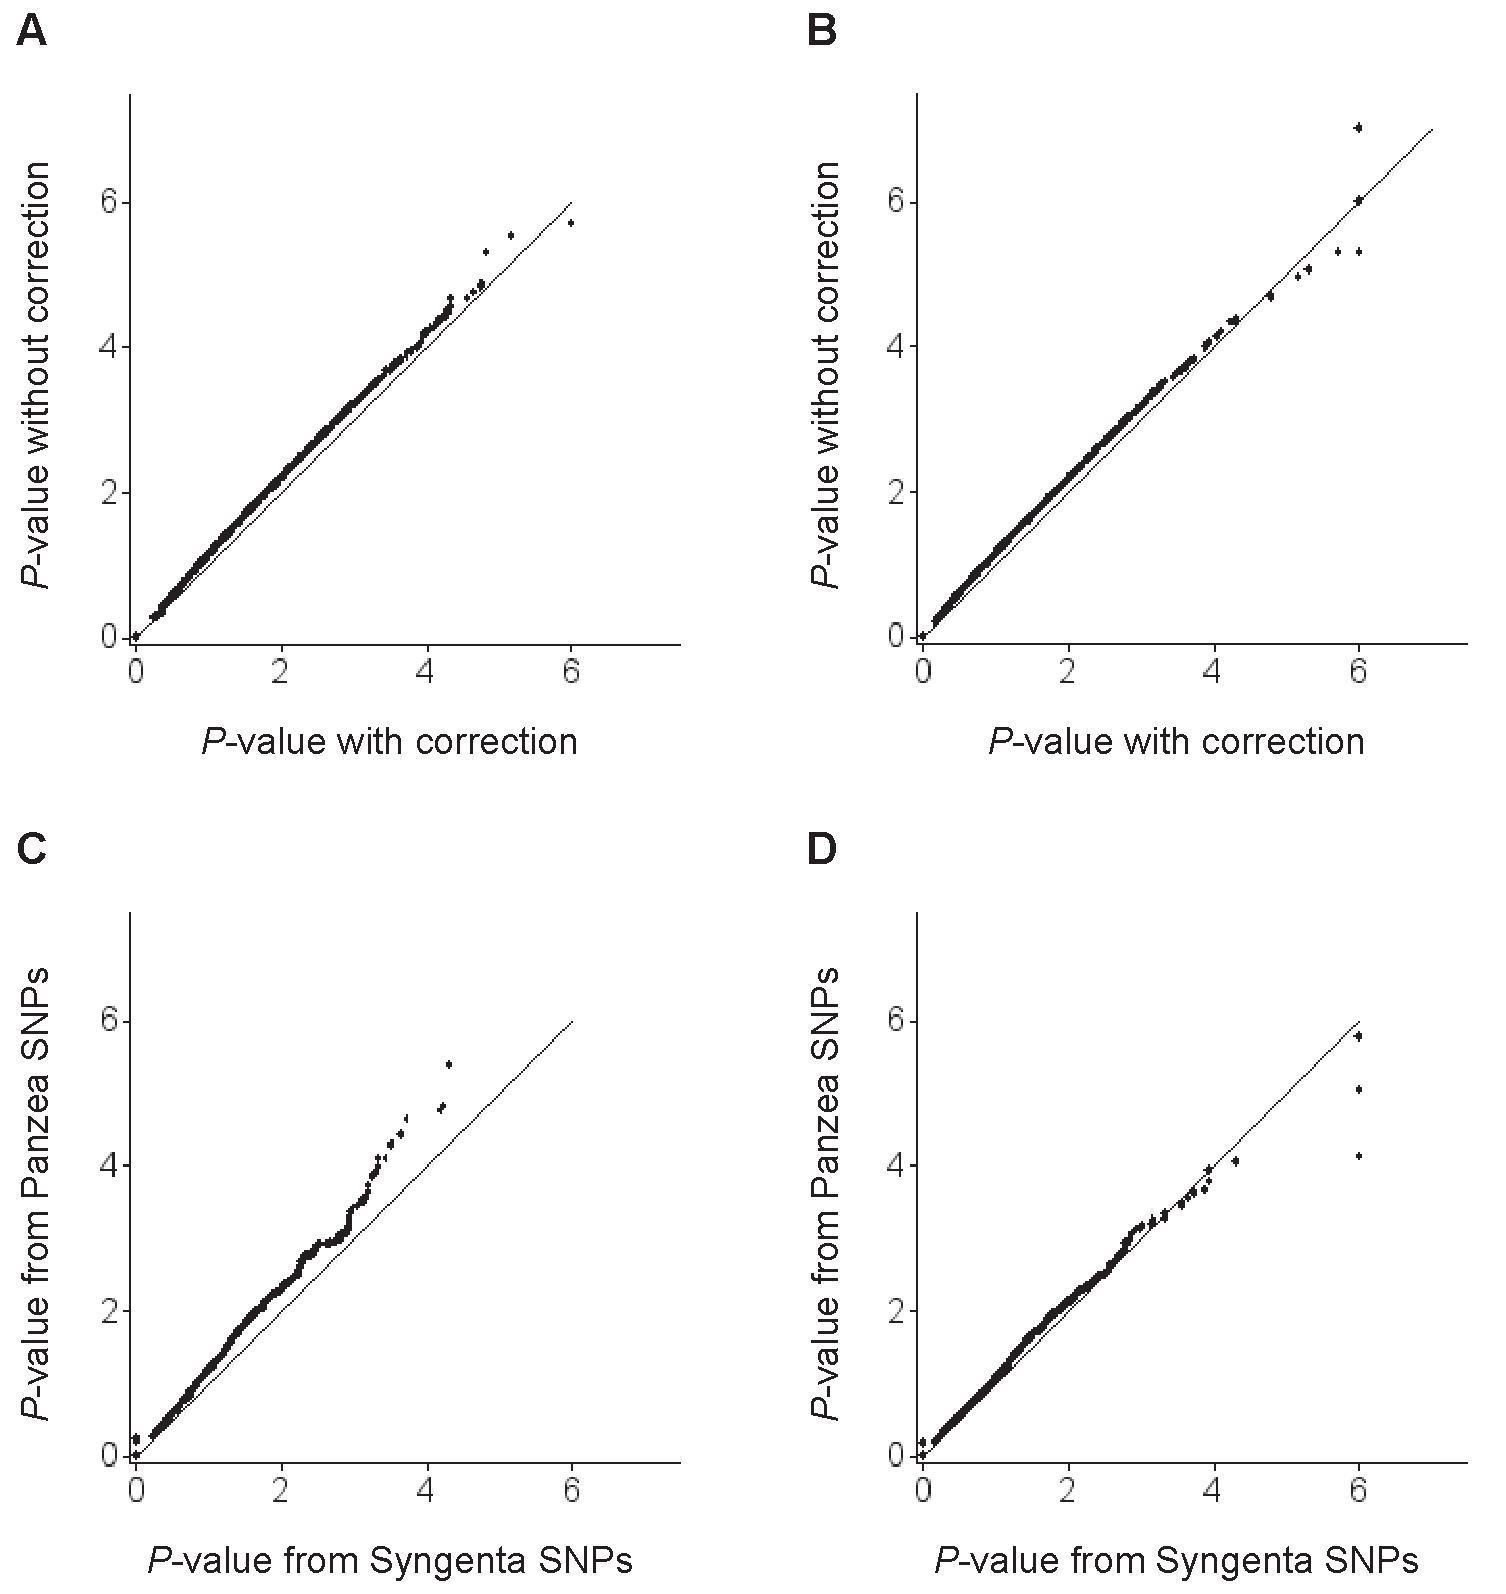
\includegraphics[width=0.6\columnwidth]{fig/MZ50P.pdf}
%    \caption{Q-Q plot for $-$log$_{10}$-scaled \emph{P}-values in MaizeSNP50 data.  (A, B) Q-Q plot of \emph{P}-values with and without correlation of ascertainment bias (on the \emph{x}- and \emph{y}-axes, respectively) in Mexico (A) and South America (B).   (C, D) Q-Q plot of \emph{P}-values from Syngenta SNPs on the \emph{x}-axes and from Panzea SNPs on the \emph{y}-axes in Mexico (C) and South America (D).  The solid lines represent \emph{y}=\emph{x}.}
%    \label{colfreq}
%  \end{center}
%\end{figure}
%%%%%%%%%%%%%%%%%%%%%%%%%%%%%%%%%%%%%%%%%%%%%%%%%%%%%%%%%%%%





%\end{document}










 

\end{document}

